%&"main"
% Fakesection 检错
% Fakesubsubsection 宏包
\RequirePackage[l2tabu, orthodox]{nag}
% Fakesubsubsection 编译器
\RequirePackage{ifxetex}
\RequireXeTeX

\documentclass[twoside, openright]{article}
% Fakesection 基础
% Fakesubsection 文字
% Fakesubsubsection 颜色
\usepackage[x11names]{xcolor}
% XXX: conflict with microtype <02-11-19> %
% Fakesubsubsection 长度
\usepackage{printlen}
\uselengthunit{mm}
% Fakesubsubsection 效果
\usepackage{ulem}
% Fakesubsubsection 字体
\usepackage{fontspec}
\setmainfont{Times New Roman}
% XXX: load ctex before siunitx to avoid \ohm ineffective <04-10-19> %
\usepackage[
	UTF8,
	fontset = windows,
	heading = true,
	zihao = -4,
	sub4section,
]{ctex}
\setCJKfamilyfont{zhsong}[
	AutoFakeBold = 2.17,
	AutoFakeSlant = 0.5,
]{SimSun}
\renewcommand*{\songti}{\CJKfamily{zhsong}}
% XXX: load newtxtext before textcomp to avoid option clash <04-10-19> %
\usepackage{newtxtext}
% Fakesubsubsection 字符边框
\usepackage{varwidth}
% Fakesubsection 断行
\usepackage{fvextra}
% Fakesubsection 标点
% XXX: load csquotes after fvextra to avoid warning <04-10-19> %
\usepackage{csquotes}
% Fakesubsubsection Unicode引号样式
\DeclareQuoteStyle{ucstyle}% style name
{\symbol{"201C}}% opening outer mark
{\symbol{"201D}}% closing outer mark
{\symbol{"2018}}% opening inner mark
{\symbol{"2019}}% closing inner mark
% Fakesubsubsection 传统中文样式
\DeclareQuoteStyle{cnzhstyle}% style name
{\symbol{"300E}}% opening outer mark
{\symbol{"300F}}% closing outer mark
{\symbol{"300C}}% opening inner mark
{\symbol{"300D}}% closing inner mark
\setquotestyle{cnzhstyle}
% Fakesubsubsection 书名号样式
\DeclareQuoteStyle{zhtitlestyle}% style name
{\symbol{"300A}}% opening outer mark
{\symbol{"300B}}% closing outer mark
{\symbol{"3008}}% opening inner mark
{\symbol{"3009}}% closing inner mark
% Fakesubsection 样式
% Fakesubsubsection 目录
\usepackage{titletoc}
\titlecontents{section}[0pt]{\filright}{\contentspush{\thecontentslabel}}{}{\titlerule*{.}\contentspage}
% Fakesubsubsection 章节
\ctexset{
	section = {
		name = ,
		number = \arabic{section},
		aftername = \hspace{1\ccwd},
		format = \ifthenelse{\value{section}=0}{\centering}{}\zihao{3}\heiti\bfseries,
		beforeskip = 0.5\ccwd,
		afterskip = 0.5\ccwd,
	},
	subsection = {
		aftername = \hspace{1\ccwd},
		format = \ifthenelse{\value{section}=0}{\centering}{}\zihao{-3}\heiti\bfseries,
		beforeskip = 0.5\ccwd,
		afterskip = 0.5\ccwd,
	},
	subsubsection = {
		format = \zihao{4}\heiti\bfseries,
	}
}
% Fakesubsubsection 图表
\usepackage{caption}
\captionsetup[figure]{labelsep=space}
\captionsetup[table]{labelsep=space}
\captionsetup{font=small}
\DeclareCaptionFont{blue}{\color{LightSteelBlue3}}
\setlength{\abovecaptionskip}{0.5\ccwd}
\setlength{\belowcaptionskip}{0.5\ccwd}
% Fakesubsubsection 子图表
\usepackage{subcaption}
% Fakesubsubsection 公式
\setlength{\abovedisplayskip}{0.5em}
\setlength{\belowdisplayskip}{0.5em}
% Fakesubsubsection 列表
\usepackage{enumitem}
\setlist[enumerate, 1]{
	fullwidth,
	label = (\arabic*),
	font = \textup,
	itemindent=2em
}
\setlist[enumerate, 2]{
	fullwidth,
	label = (\alph*),
	font = \textup,
	itemindent=4em
}
% Fakesubsubsection 代码
% XXX: need -shell-escape & pygmentize <04-10-19> %
\usepackage{minted}
\usepackage{boxie}
% XXX: conflict with fancybox <02-11-19> %
% Fakesubsubsection 问答
\usepackage{exercise}
\usepackage{tasks}
% Fakesubsubsection 改动

% Fakesection 插入
% Fakesubsection 表格
% Fakesubsubsection 三线
\usepackage{booktabs}
% Fakesubsubsection 对角线
\usepackage{diagbox}
% Fakesubsubsection 合并列
\usepackage{multicol}
% Fakesubsubsection 合并行
\usepackage{multirow}
% Fakesubsubsection 分割单元格
\usepackage{makecell}
% Fakesubsubsection 短表
\usepackage{tabu}
% Fakesubsubsection 长表
\usepackage{longtable}
% Fakesubsubsection 彩色表
\usepackage{colortbl}
\usepackage{tcolorbox}
\tcbuselibrary{skins}
\tcbuselibrary{breakable}
\tcbuselibrary{theorems}
\tcbuselibrary{listings}
\tcbuselibrary{xparse}
% XXX: need -shell-escape & pygmentize <04-10-19> %
\tcbuselibrary{minted}
% Fakesubsubsection 导入数据
\usepackage{csvsimple}
% Fakesubsection 图形
% Fakesubsubsection 插图
\usepackage{graphicx}
\graphicspath{{fig/}{etc/}}
% Fakesubsubsection 环绕
\usepackage{wrapfig}
% Fakesubsubsection 图片重叠
\usepackage{overpic}
% Fakesubsubsection 徽标
\usepackage{hologo}
% Fakesubsubsection 条形码
\usepackage{ean13isbn}
% Fakesubsubsection 二维码
\usepackage{qrcode}
% Fakesubsection 符号
% Fakesubsubsection 数学符号
\usepackage{newtxmath}
\usepackage{bm}
% Fakesubsubsection 幻灯片符号
\usepackage{pifont}
% Fakesubsubsection 大数学符号
\usepackage{exscale}
% Fakesubsubsection 数学符号放缩
\usepackage{relsize}
% Fakesubsubsection 公式
\usepackage{cases}
\usepackage{physics}
% Fakesubsubsection 单位
\usepackage{siunitx}
\sisetup{mode=text}
% Fakesubsubsection 计算机
% Fakesubsubsection 音乐
\usepackage{mtxlatex}
\mtxlatex
% Fakesubsection 媒体
\usepackage{media9}
% Fakesubsection 链接
\usepackage[
	colorlinks = true,
	linkcolor = gray,
	citecolor = gray,
	backref = page
]{hyperref}
% Fakesubsection 批注
\usepackage{todonotes}
\usepackage{cooltooltips}
\usepackage{pdfcomment}
% Fakesubsection 文本框
\usepackage{boxedminipage2e}
% Fakesubsection 页眉页脚
\usepackage{fancyhdr}
\fancypagestyle{plain}{
	\pagestyle{fancy}
}

% Fakesection 设计
% Fakesubsection 水印
\usepackage{wallpaper}
% Fakesubsection 主题

% Fakesection 布局
% Fakesubsection 页面
\usepackage{geometry}
% Fakesubsection 缩进
\usepackage{indentfirst}
% Fakesubsection 间距
\usepackage{setspace}
\usepackage[
	restoremathleading=false,
	UseMSWordMultipleLineSpacing,
	MSWordLineSpacingMultiple=1.5
]{zhlineskip}
% Fakesection 引用
% Fakesubsection 脚注
\renewcommand{\thefootnote}{\fnsymbol{footnote}}
\renewcommand{\thempfootnote}{\fnsymbol{mpfootnote}}
% Fakesubsection 引文
\usepackage{morewrites}
\usepackage[square, comma, numbers, super, sort&compress, longnamesfirst, sectionbib, nonamebreak]{natbib}
% Fakesubsection 题注
\usepackage{epigraph}
% Fakesubsection 索引
\usepackage{makeidx}
\makeindex
% Fakesubsection 关联
% XXX: need amsmath <04-10-19> %
%\numberwithin{Exercise}{chapter}
%\numberwithin{Answer}{chapter}

% Fakesection 特殊功能
% Fakesubsection 页数统计
\usepackage{lastpage}
% Fakesubsection 数学表达式
\usepackage{calc}

\begin{document}

% Fakesection 扉页

\newcommand{\Title}{EDA设计实验报告}

\begin{titlepage}
	\centering
	\begin{spacing}{1}
		\zihao{4}
		\vspace{0.5\ccwd}

		\vspace{1\ccwd}

		\includegraphics[width=7.41cm]{NJUST.ai}

		\vspace{0.2\ccwd}

		\fontsize{45pt}{45pt}\selectfont\heiti
		\Title

		\zihao{-1}
		\vspace{2\ccwd}
	\end{spacing}

	\begin{spacing}{1.5}
		\zihao{3}
		\begin{tabu} to 12.59cm{@{}X[c, 3.2cm]@{}X[c, 4cm]@{}X[c, 2.22cm]@{}X[c, 3.89cm]@{}}
			\textbf{作  者:} & \underline{\makebox[4cm][c]{\kaishu 吴振宇}} & \textbf{学 号:} & \underline{\makebox[3.89cm][c]{\kaishu 916101630117}} \\
			\textbf{学  院:} & \multicolumn{3}{c}{\underline{\makebox[10.11cm][c]{\kaishu 电子工程与光电技术学院}}} \\
			\textbf{专业(方向):} & \multicolumn{3}{c}{\underline{\makebox[10.11cm][c]{\kaishu 电子信息工程}}} \\
			\textbf{班  级:} & \multicolumn{3}{c}{\underline{\makebox[10.11cm][c]{\kaishu 电信4班}}} \\
			\textbf{题  目:} & \multicolumn{3}{c}{\underline{\makebox[10.11cm][c]{\kaishu 多功能数字时钟设计}}} \\
			\textbf{} & \multicolumn{3}{c}{\underline{\makebox[10.11cm][c]{\kaishu}}}
		\end{tabu}
		\vspace{0em}
	\end{spacing}

	\begin{spacing}{1}
		\zihao{3}
		\vspace{3\ccwd}

		\zihao{-3}
		\textbf{指导者:}\underline{\makebox[15.5\ccwd][c]{}}

		\zihao{5}
		\hspace{5em}(姓名)\hspace{11em}(专业技术职务)

		\zihao{-3}
		    \underline{\makebox[15.5\ccwd][c]{}}

		\zihao{5}
		\hspace{5em}(姓名)\hspace{11em}(专业技术职务)

		\zihao{-3}
		\textbf{评阅者:}\underline{\makebox[15.5\ccwd][c]{}}

		\zihao{5}
		\hspace{5em}(姓名)\hspace{11em}(专业技术职务)

		\zihao{3}
		\vspace{2\ccwd}

		\zihao{-2}
		\number\year 年\number\month 月
	\end{spacing}
	\vspace{0em}
\end{titlepage}

% Fakesection 声明

\renewcommand{\abstractname}{\zihao{3}\heiti 声\hspace{2\ccwd}明}
\begin{abstract}
	\zihao{4}

	我声明,本\Title 及其研究工作和所取得的成果是本人在导师的指导下独立完成
	的。研究过程中利用的所有资料均已在参考文献中列出,其他人员或机构对本
	\Title 工作做出的贡献也已在致谢部分说明。

	本\Title 不涉及任何秘密,南京理工大学有权保存其电子和纸质文档,可以借阅
	或网上公布其部分或全部内容,可以向有关部门或机构送交并授权保存、借阅或网
	上公布其部分或全部内容。

	\vspace{2\ccwd}

	\begin{flushright}
		学生签名:\hspace{8em}

		\vspace{1\ccwd}

		年\hspace{3em}月\hspace{3em}日

		\vspace{2\ccwd}

		指导教师签名:\hspace{8em}

		\vspace{1\ccwd}

		年\hspace{3em}月\hspace{3em}日
	\end{flushright}
\end{abstract}

% Fakesection 摘要页眉页脚

\pagestyle{fancy}
\renewcommand{\headrulewidth}{0pt}
\fancyhead[LC, RC]{}
\fancyhead[LE, RO]{}
\fancyhead[RE, LO]{}
\fancyfoot[LC, RC]{}
\fancyfoot[LE, RO]{}
\fancyfoot[RE, LO]{}

% Fakesection 摘要

\newpage

\begin{center}
	\zihao{3}\renewcommand{\CJKglue}{\hskip 2pt}\heiti \Title 中文摘要

	\vspace{0.3em}

	\begin{boxedminipage}[][18cm]{\linewidth}
		\begin{spacing}{1.5}
			\zihao{-4}

			\vspace{1\ccwd}

			本实验利用 QuartusII 软件设计一个多功能数字计时器,并下
			载到 SmartSOPC 实验系统中。这个数字计时器,可以完成
			00:00:00 到 23:59:59 的计时功能,并在控制电路的作用下具
			有保持、清零、快速校时、快速校分、整点报时等功能,这些
			功能相互独立,却又互相协调配合。在此类基础功能之上还添
			加了显示星期、闹钟、秒表、彩铃功能。
			\cite{姜萍2008创新教育在, 2010数字逻辑电路基础, 孙敦艳2011硬件描述语言在数字逻辑电路教学中的应用}

			\vspace{2\ccwd}

			\noindent\textbf{关键词}\hspace{1\ccwd}多功能数字钟\hspace{1\ccwd}SmartSOPC\hspace{1\ccwd}QuartusII
		\end{spacing}
	\end{boxedminipage}
\end{center}

% Fakesection 英文摘要

\newpage

\begin{center}
	\zihao{3}\renewcommand{\CJKglue}{\hskip 2pt}\heiti \Title 英文摘要

	\vspace{0.3em}

	\begin{boxedminipage}[][18cm]{\linewidth}
		\begin{spacing}{1.5}
			\zihao{3}

			\vspace{1em}

			\begin{tabu} to \linewidth{@{}X[l]@{}X[l, 8]@{}}
				\textbf{Title} & \hspace{2em}\underline{\makebox[15em][c]{\zihao{4}\songti Multi-functional Digital Timer}} \\
					       & \hspace{2em}\underline{\makebox[15em][c]{\zihao{4}\songti }} \\
			\end{tabu}

			\textbf{Abstract}

			\zihao{-4} In this experiment, QuartusII software is
			used to design a multi-functional digital timer, which
			is downloaded to the smartsopc experimental system.
			This digital timer can complete the timing function from
			00:00:00 to 23:59:59. Under the control circuit, it has
			the functions of keeping, clearing, fast time
			calibration, fast time calibration and whole time
			reporting. These functions are independent of each
			other, but coordinated with each other. In addition to
			such basic functions, has added displaying week, alarm
			clock, stopwatch and polyphonic ringtone.

			\vspace{2em}

			\noindent\textbf{Keywords}\hspace{1em}multi-functional digital timer\hspace{1em}SmartSOPC\hspace{1em}QuartusII
		\end{spacing}
	\end{boxedminipage}
\end{center}

% Fakesection 目录页眉页脚

\newpage

\renewcommand{\headrulewidth}{0.4pt}
\fancyhead[LC, RC]{\zihao{-2}\Title}
\fancyhead[LE, RO]{\zihao{5}第\thepage 页}
\fancyhead[RE, LO]{}

% Fakesection 目录

\pagenumbering{roman}

\setcounter{tocdepth}{2}

\renewcommand{\contentsname}{\zihao{3}\heiti 目次}
\tableofcontents
\listoffigures
\listoftables

\newpage
\pagenumbering{arabic}

% Fakesection 正文

\section{实验要求}%
\label{sec:实验要求}

\subsection{实验基本要求}%
\label{sub:实验基本要求}

\begin{enumerate}

	\item 能进行正常的时、分、秒计时功能;

	\item $ K_1 $是系统的使能开关($ K_1 = 0$正常工作,$ K_1 = 1$数字钟保持
		不变);

	\item $ K_2 $是系统的清零开关($ K_2 = 0$正常工作,$ K_2 = 1$数字钟全清
		零);

	\item $ K_3 $是系统的校分开关($ K_3 = 0$正常工作,$ K_3 = 1$时可以快速
		校分);

	\item $ K_4 $是系统的校时开关($ K_4 = 0$正常工作,$ K_4 = 1$时可以快速
		校时);

	\item 使数字钟具有整点报时功能(当数字钟计到\ang{;59;53}时开始报时,在
		\ang{;59;53}\ang{;59;55}\ang{;59;57}时报时频率为
		\SI{500}{\Hz};\ang{;59;59}时报时频率为\SI{1}{\kHz})。

\end{enumerate}

\subsection{实验提高要求}%
\label{sub:实验提高要求}

\begin{enumerate}

	\item 添加星期功能;

	\item 万年历功能;

	\item 闹表设定功能;

	\item 秒表功能;

	\item 自己添加其他功能;

	\item 彩铃功能。

\end{enumerate}

\section{子模块设计及原理图}%
\label{sec:子模块设计及原理图}

根据实验要求章节\ref{sec:实验要求},一共有如下6大子电路,其相互关系见图
\ref{fig:电路整体框图}。

\begin{figure}[htbp]
	\centering
	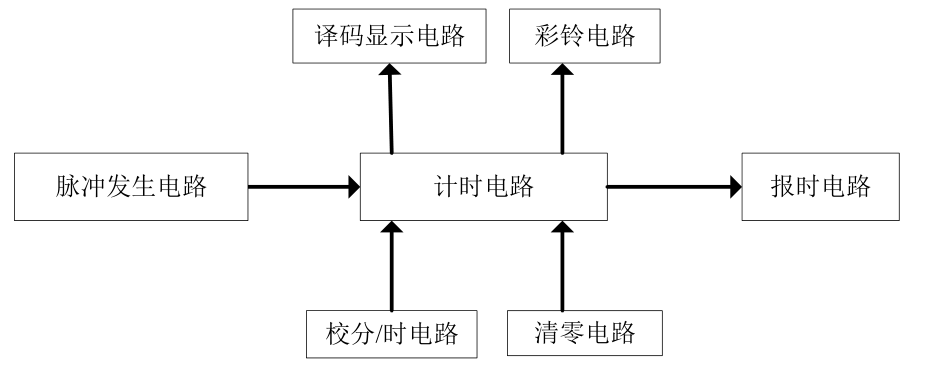
\includegraphics[width=0.8\linewidth]{block.png}
	\caption{电路整体框图}
	\label{fig:电路整体框图}
\end{figure}

按功能可进一步细分为以下部分:

\begin{description}

	\item[\nameref{sub:脉冲发生电路}:] 通过对主时钟进行分频,产生\SI{1}{\kHz},
		\SI{500}{\Hz}, \SI{2}{\Hz}, \SI{1}{\Hz}等电路所需要的时钟频率;

	\item[\nameref{sub:计时电路}:] 采用计数器组成,对\SI{1}{\Hz}信号进行计数,是整个电路的
		核心;

	\item[\nameref{sub:校分/时电路}:] 快速调整分钟/小时,以便对电路进行检测;

	\item[\nameref{sub:计数保持电路}:] 保持计数值不变;

	\item[\nameref{sub:清零电路}:] 将所有计数器清零,用以检测电路;

	\item[\nameref{sub:消抖电路}:] 接在按键输入端后,以消除抖动;

	\item[\nameref{sub:显示译码电路}:] 将计数器的输出数字翻译成数码管的显示数字,并采用
		\SI{1}{\kHz}信号使数码管动态显示;

	\item[\nameref{sub:报时电路}:] 当计数器数值达到预定值的时候,蜂鸣器响起,达到类似闹钟的
		效果;

	\item[\nameref{sub:闹钟电路}:] 开关复用后,通过定时定分设定闹铃的预定时
		间;

	\item[\nameref{sub:彩铃电路}:] 到达闹铃的预定时间,蜂鸣器的报时信号为音乐;

	\item[\nameref{sub:秒表电路}:] 显示从0开始经过的时间。

\end{description}

\subsection{脉冲发生电路}%
\label{sub:脉冲发生电路}

实验中提供稳定的频率为\SI{48}{\MHz}的高频脉冲,需使用到系统时钟\SI{1}{\Hz}、报时
电路中蜂鸣器使用的\SI{2}{\kHz}、\SI{1}{\kHz}频率,故需要将时钟信号分频。

\begin{figure}[htbp]
	\centering
	\begin{subfigure}[htbp]{.45\linewidth}
		\centering
		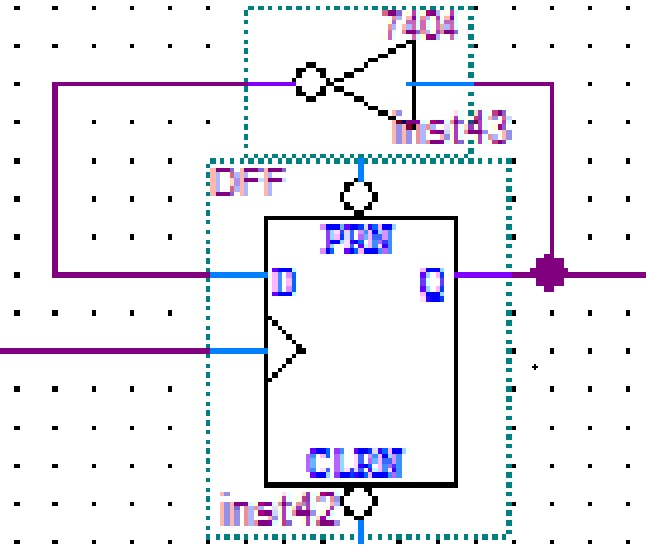
\includegraphics[width=\linewidth]{2.jpg}
		\caption{2分频}
		\label{fig:2分频}
	\end{subfigure}
	\quad
	\begin{subfigure}[htbp]{.45\linewidth}
		\centering
		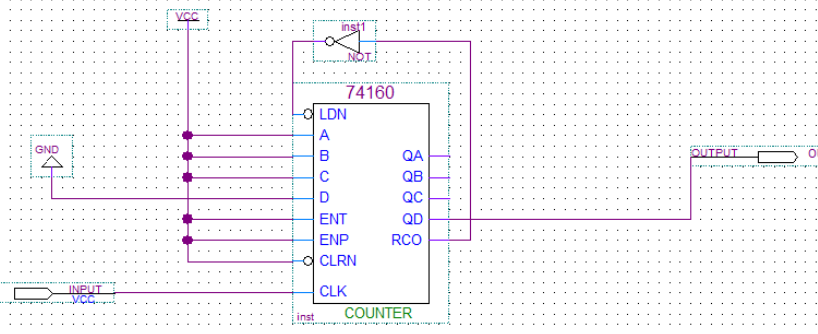
\includegraphics[width=\linewidth]{3.png}
		\caption{3分频}
		\label{fig:3分频}
	\end{subfigure}

	\begin{subfigure}[htbp]{.45\linewidth}
		\centering
		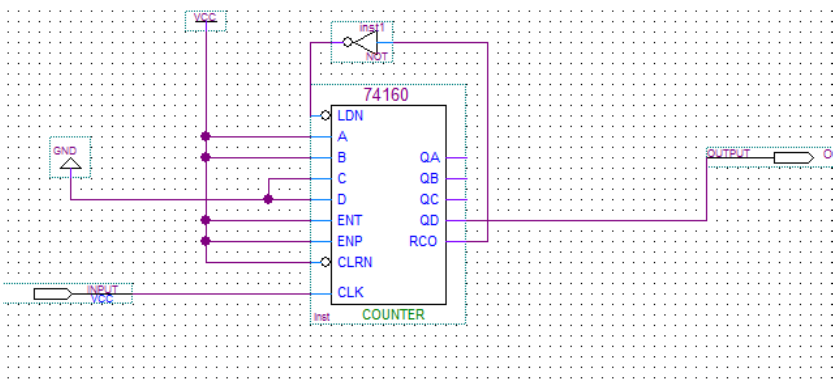
\includegraphics[width=\linewidth]{7.png}
		\caption{7分频}
		\label{fig:7分频}
	\end{subfigure}
	\quad
	\begin{subfigure}[htbp]{.45\linewidth}
		\centering
		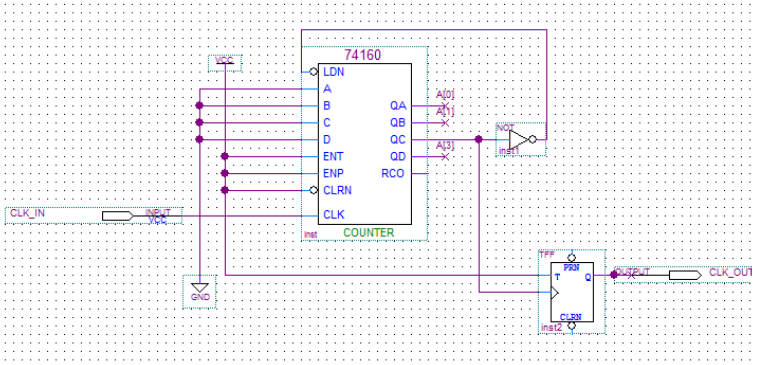
\includegraphics[width=\linewidth]{10.png}
		\caption{10分频}
		\label{fig:10分频}
	\end{subfigure}

	\caption{分频电路}
	\label{fig:分频电路}
\end{figure}

如图\ref{fig:2分频},二分频器采用一个 D 触发器和一个非门组成 T 触发器,其状态方
程为:

\begin{align}
	Q^{n + 1} = Q^n
\end{align}

每当一个上升沿到来,计数器翻转一次,可对输入信号进行二分频。

如图\ref{fig:3分频},采用模十计数器 74160 组成模 3 计数器,其有效状态有 0111,
1000,1001,当计数到 1001 时,输出端 RCO 输出信号到计数器置数端,使计数器回到状
态 0111。经过分频后的输出信号为计数值的高位。仿真波形图如图\ref{fig:3分频仿真}。

如图\ref{fig:7分频},与三分频电路类似,采用计数器 74160 和非门组成模 7 计数器,
采用置数法,其有效状态共 7 种:0011,0100,0101,0110,0111,1000,1001。当电路计数到
1001 时,RCO 端发出置数信号,使计数器回到初始状态。由最高位 QD 取出信号,得到经
过 7 分频之后的时钟信号。仿真波形图如图\ref{fig:7分频仿真}。七分频电路方便进行星
期的显示。

如图\ref{fig:10分频},采用模十计数器 74160 构成模 5 计数器,再添加一个 T 触发器
构成二分频器便得到了 10 分频器,其有效状态有:0000,0001,0010,0011,0100。仿真波形
图如图\ref{fig:10分频仿真}。

\begin{figure}[htbp]
	\centering
	\begin{subfigure}[htbp]{.31\linewidth}
		\centering
		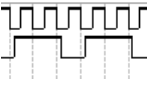
\includegraphics[width = \linewidth]{3-2.png}
		\caption{3分频仿真}
		\label{fig:3分频仿真}
	\end{subfigure}
	\quad
	\begin{subfigure}[htbp]{.31\linewidth}
		\centering
		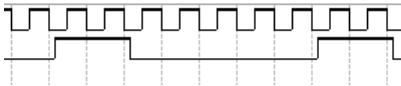
\includegraphics[width = \linewidth]{7-2.png}
		\caption{7分频仿真}
		\label{fig:7分频仿真}
	\end{subfigure}
	\quad
	\begin{subfigure}[htbp]{.31\linewidth}
		\centering
		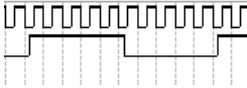
\includegraphics[width = \linewidth]{10-2.png}
		\caption{10分频仿真}
		\label{fig:10分频仿真}
	\end{subfigure}
	\caption{分频仿真}
	\label{fig:分频仿真}
\end{figure}

总的原理图如图\ref{fig:分频原理图}。

\begin{figure}[htbp]
	\centering
	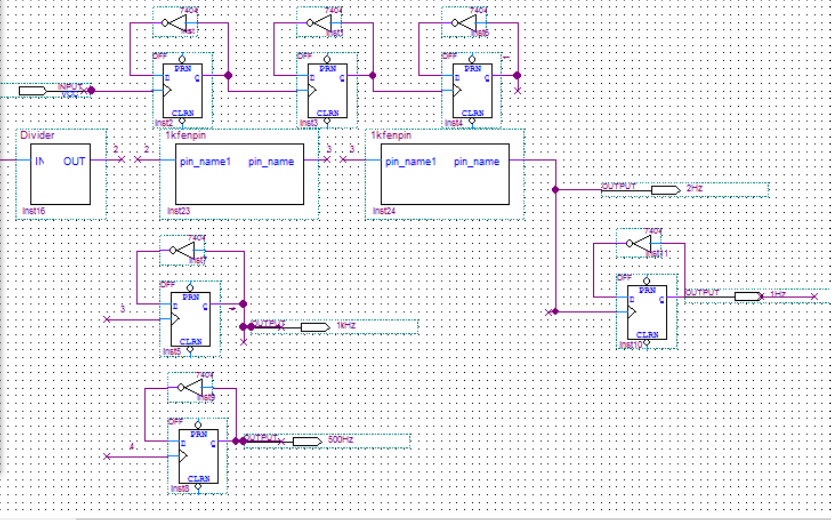
\includegraphics[width = 0.8\linewidth]{divider.png}
	\caption{分频原理图}
	\label{fig:分频原理图}
\end{figure}

可以看到用原理图搭建电路繁琐麻烦。可以考虑使用硬件描述语言对电路进行行为级建模。
思路为:对时钟信号进行上升沿检测,并记录检测的数(从 0 开始计数)。如果是$ N $分
频,每当计数到$ \dfrac{N}{2} - 1 $时将信号翻转一次,将信号输出。

\langCVfile[verilog][lst:divider.v][verilog]{divider.v}{lst/divider.v}

\langCVfile[verilog][lst:divider.vt][verilog]{divider.vt}{lst/divider.vt}

\subsection{计时电路}%
\label{sub:计时电路}

如图\ref{fig:计时电路}所示,秒个位在输入时钟信号上升沿时进行计数,其值从0000到
1001循环。在计时过程中,当秒个位的状态由1001变为0000时,秒十位接收一个进位信号来
实现进位,该信号为秒个位的下降沿(由“1”到“0”的变化),从而实现进位。同理可得秒十
位向分个位的进位信号。

\begin{figure}[htbp]
	\centering
	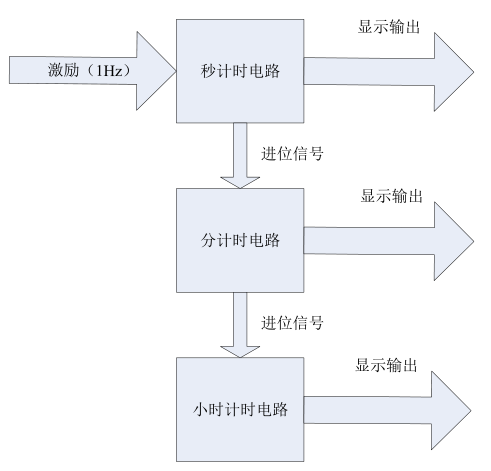
\includegraphics[width = 0.6\linewidth]{count.png}
	\caption{计时电路}
	\label{fig:计时电路}
\end{figure}

秒计数器的模为 60,电路上采用十进制计数器 74160 构成一个模 10 计数器和一个模 6
计数器,再将两者接在同一计数脉冲上,可得到模 60 计数器。

\begin{figure}[htbp]
	\centering
	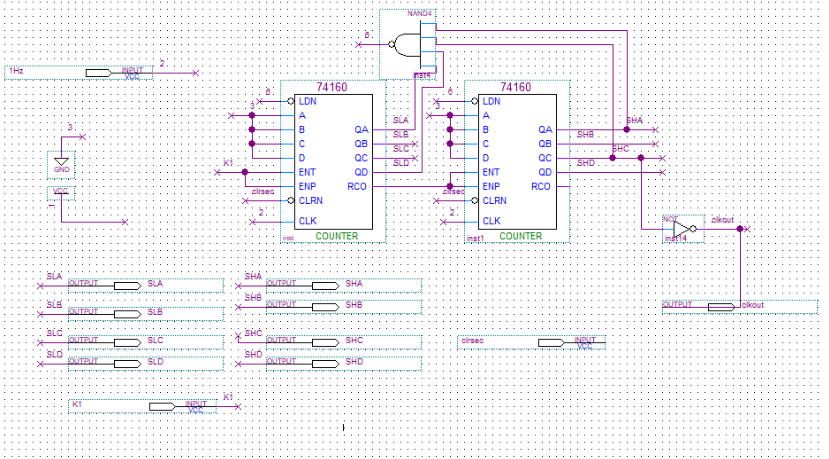
\includegraphics[width = 0.8\linewidth]{sec.png}
	\caption{秒/分计时电路}
	\label{fig:秒/分计时电路}
\end{figure}

\begin{figure}[htbp]
	\centering
	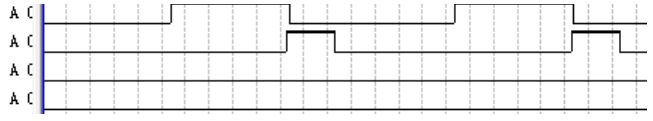
\includegraphics[width = 0.8\linewidth]{sec-1.png}
	\caption{秒/分计时电路低位仿真波形}
	\label{fig:秒/分计时电路低位仿真波形}
\end{figure}

\begin{figure}[htbp]
	\centering
	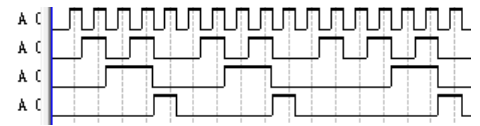
\includegraphics[width = 0.8\linewidth]{sec-2.png}
	\caption{秒/分计时电路高位仿真波形}
	\label{fig:秒/分计时电路高位仿真波形}
\end{figure}

如图\ref{fig:秒/分计时电路} 所示,左边计数器为低位的模十计数器,每来一个脉冲计数
值加一,其计数状态为 0 到 9 。低位计数器的 RCO 端接到高位计数器的 ENT、ENP,低位
计数值为 0 到 8 时,高位计数器停止计数。当低位计数器计数值为 9 时,RCO 端输出变
为高电平,高位计数器被使能,当下一个脉冲到来时,高位加一计数,达到计数进位的功能
,而此时低位由最大值变为最小值。

当清零输入端接入逻辑 0 时,电路计数值被清零;$ K_1 $为计数保持端,当该端口接入逻
辑 0 的时候,计数器保持当前数值,且忽略输入的脉冲信号。右方各端口分别表示秒高位
和低位的四个计数端 A、B、C、D,可接入动态显示用。

图\ref{fig:秒/分计时电路低位仿真波形}中秒计数的低位仿真波形状态为:0000 0001
0010 0011 0100 0101 0110 0111 1000 1001,为十进制的 0 到 9 共计 10 个状态。图
\ref{fig:秒/分计时电路高位仿真波形}中秒计数高位的仿真波形状态为:0000 0001 0010
0011 0100 0101 ,为十进制的 0 到 5,共计 6 个状态。可见,该电路满足模为 60 的秒
计数电路。分计数电路与秒计数电路同理。

\begin{figure}[htbp]
	\centering
	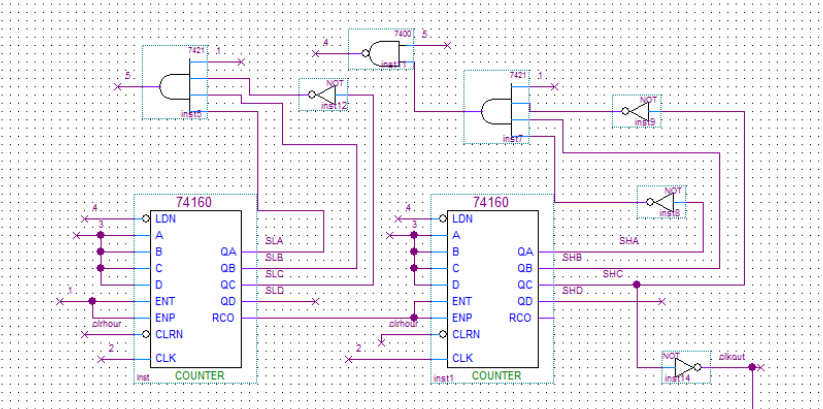
\includegraphics[width = 0.8\linewidth]{min.png}
	\caption{时计时电路}
	\label{fig:时计时电路}
\end{figure}

\begin{figure}[htbp]
	\centering
	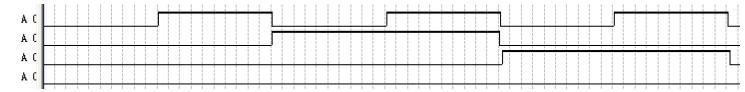
\includegraphics[width = 0.8\linewidth]{min-1.png}
	\caption{时计时电路低位仿真波形}
	\label{fig:时计时电路低位仿真波形}
\end{figure}

\begin{figure}[htbp]
	\centering
	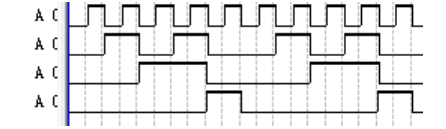
\includegraphics[width = 0.8\linewidth]{min-2.png}
	\caption{时计时电路高位仿真波形}
	\label{fig:时计时电路高位仿真波形}
\end{figure}

时计数器为模 24 。电路上采用两个模十计数器 74160 构成。当小时的高位为 0 或 1 两
种情况时,小时的低位按模 10 计数,有效状态为从 0 到 9 ;当小时的高位为 2 时,小
时的低位按模 4 计数,有效状态为从 0 到 3;由图\ref{fig:时计时电路}可知,同步置数
端信号有效的条件是:低位计数值为 0011 ,高位计数值为 0010,即计数器计数到 23 时
,下一个脉冲的上升沿使两个计数器回到 0000 的状态,达到模 24 计数的功能。

时计数器除了接小时位的清零开关、分钟计数的进位信号、小时的保持开关和小时快速计数
的输入脉冲外,小时高位和低位的 4 个计数位 A B C D 可接入动态显示端口用以动态显示
。图\ref{fig:时计时电路低位仿真波形}为小时计数电路的个位仿真波形图,可见在前两个
周期,其计数状态由 0000 到 1001 ,为十进制的 0 到 9。 在第三个周期,其计数状态变
为从 0000 到 0011 ,为十进制的 0 到 3 ;对于图 \ref{fig:时计时电路高位仿真波形}
为小时计数的十位仿真波形图,其计数状态为 0000 到 0010,为十进制的 0 到 2。满足小
时计数的要求。

\subsection{校分/时电路}%
\label{sub:校分/时电路}

实现校准时,校准信号为1,此时,若校秒信号为1,则秒个位输入时钟应该为\SI{1}{\Hz}信
号以进行校秒,若快速校秒信号为1,则秒个位输入时钟应该为\SI{2}{\Hz}信号以进行快速
校秒。

\begin{figure}[htbp]
	\centering
	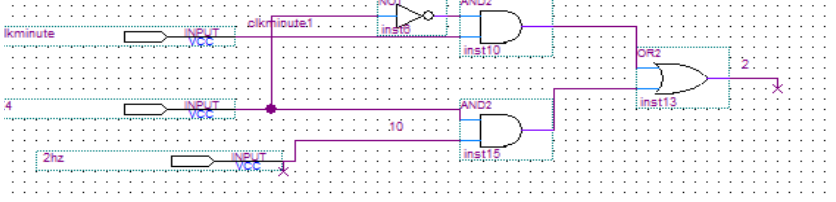
\includegraphics[width = 0.8\linewidth]{calibrate.png}
	\caption{校准电路}
	\label{fig:校准电路}
\end{figure}

图\ref{fig:校准电路}所示是校分(校时)电路原理图。当开关拨下时,分计数器和小时计
数器的输入频率被切换到\SI{2}{\Hz},原计数进位信号被屏蔽,从而实现快速校分(校时
)的功能。当开关拨回原位置的时候,电路的输入脉冲回到\SI{1}{\Hz}的正常计数模式,
其中秒位不设快速计数功能。如图所示,$ K_4 $端是校分(校时)的开关端口,当$ K_4 =
1 $时,与\SI{2}{\Hz}的输入频率相与,经过或门,\SI{2}{\Hz}信号给入计数器的时钟端
口,当$ K_4 = 0 $时,\SI{2}{\Hz}的输入经与门被置零,$ K_4 $经过非门,与秒计数器
或分计数器的进位端相与,之后经过或门送入分(时)计数器的时钟端,从而在$ K_4 = 0
$ 时正常计数。

\subsection{计数保持电路}%
\label{sub:计数保持电路}

\begin{wrapfigure}{r}{0.6\linewidth}
	\centering
	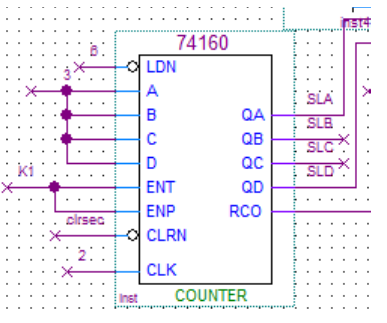
\includegraphics[width = \linewidth]{keep.png}
	\caption{计数保持电路}
	\label{fig:计数保持电路}
	\vspace{-4em}
\end{wrapfigure}

如图\ref{fig:计数保持电路}所示,保持电路的实现依赖于计数器本身的保持端口 ENT、
ENP,当保持端接 1 时,计数器正常计数;当保持端接 0 时,计数器会忽略时钟端口到来
的脉冲信号,保持现有的数值不变。同清零电路一样,保持电路也有消抖电路作为中间缓冲
区消除机械抖动。

\subsection{清零电路}%
\label{sub:清零电路}

如图\ref{fig:清零电路}所示,清零电路是在任何状态下将电路归零的电路,由$ U_4 $控
制,$ U_4 = 1 $时,各个位的数字置0 。

\begin{figure}[htbp]
	\centering
	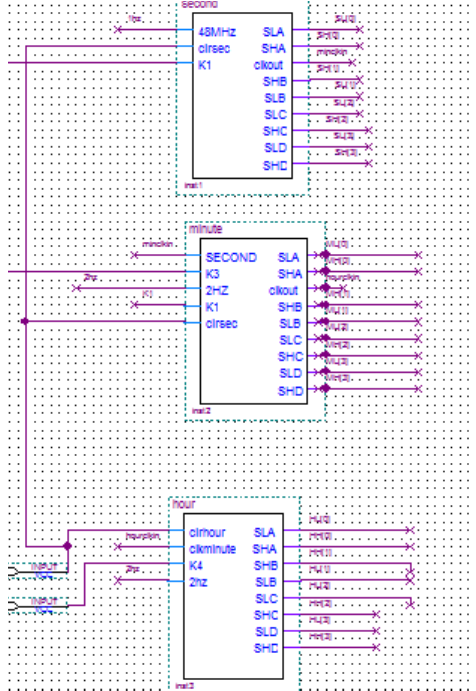
\includegraphics[width = 0.6\linewidth]{clear.png}
	\caption{清零电路}
	\label{fig:清零电路}
\end{figure}

\subsection{消抖电路}%
\label{sub:消抖电路}

如图\ref{fig:消抖电路}所示,将开关连接到 D 触发器的输入端。以清零开关为例,当开
关处于拨下状态时,计数器清零端有效,计时器数值清零。而在开关拨下的过程中,由于机
械抖动,开关输入到计数器的信号是不稳定的,将会导致计数器的数值不断乱跳。将其接入
D 触发器后,颤抖明显被消除,输入信号稳定性得到改善。

\begin{figure}[htbp]
	\centering
	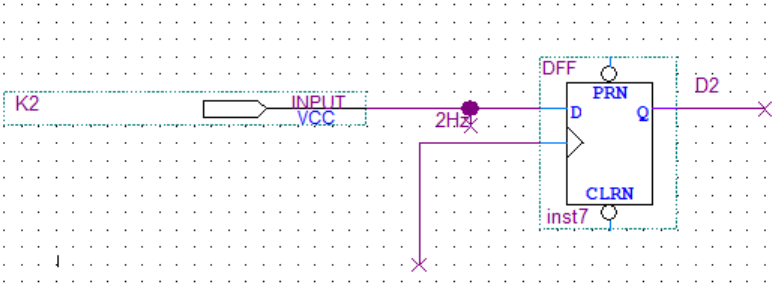
\includegraphics[width = 0.6\linewidth]{tremble.png}
	\caption{消抖电路}
	\label{fig:消抖电路}
\end{figure}

\subsection{显示译码电路}%
\label{sub:显示译码电路}

动态扫描是把所有显示器的8个段码中的a-dp的各个相同段连接在一起, 接到一个公共的输
出口上,而数码管的位端分别接在另外的输出口上,通过这两个输出口的两组信号相互作用
来产生显示效果。即让各位数码管按照一定顺序轮流显示, 只要扫描频率足够高, 由于人
眼的“视觉暂留”现象,就能连续稳定的显示。本次实验中选择了\SI{1}{\kHz}。

\begin{figure}[htbp]
	\centering
	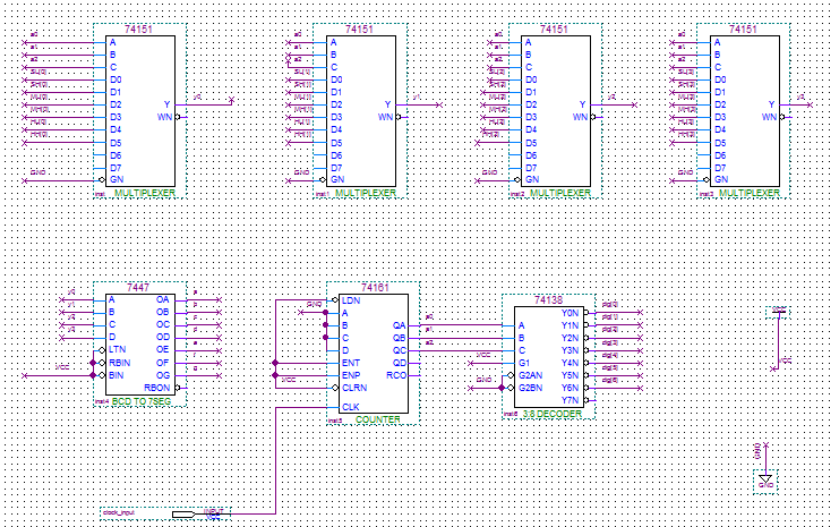
\includegraphics[width = 0.8\linewidth]{display.png}
	\caption{显示译码电路}
	\label{fig:显示译码电路}
\end{figure}

按照高电平对应的数码管被点亮的工作方式, 该数码管为阳极驱动。如图
\ref{fig:显示译码电路},四个 8 选 1 数据选择器 74151 一起组成了 24 选 4 数据选择
器(每个数据选择器只使用了 6 位),将 6 个数字轮流送到数码管译码器 7474 进行译码
显示。74138 为译码器,用于点亮数字所对应的数码管。输入\SI{1}{\kHz}的刷新频率用于
动态显示。

\subsection{报时电路}%
\label{sub:报时电路}

报时电路要求在每个小时里,分钟位和秒位计数达到 59 分 53 秒,59 分 55 秒,59 分
57 秒时,蜂鸣器输出低频信号声音,在 59 分 59 秒蜂鸣器输出高频信号声音。将四种情
况列于表\ref{tab:报时电路}:

\begin{table}[htbp]
	\centering
	\caption{报时电路}
	\label{tab:报时电路}
	\csvautobooktabular{tab/give-time.csv}
\end{table}

画出卡诺图如图\ref{fig:卡诺图}\footnote{X表示其中的无效状态}。

\begin{figure}[htbp]
	\centering
	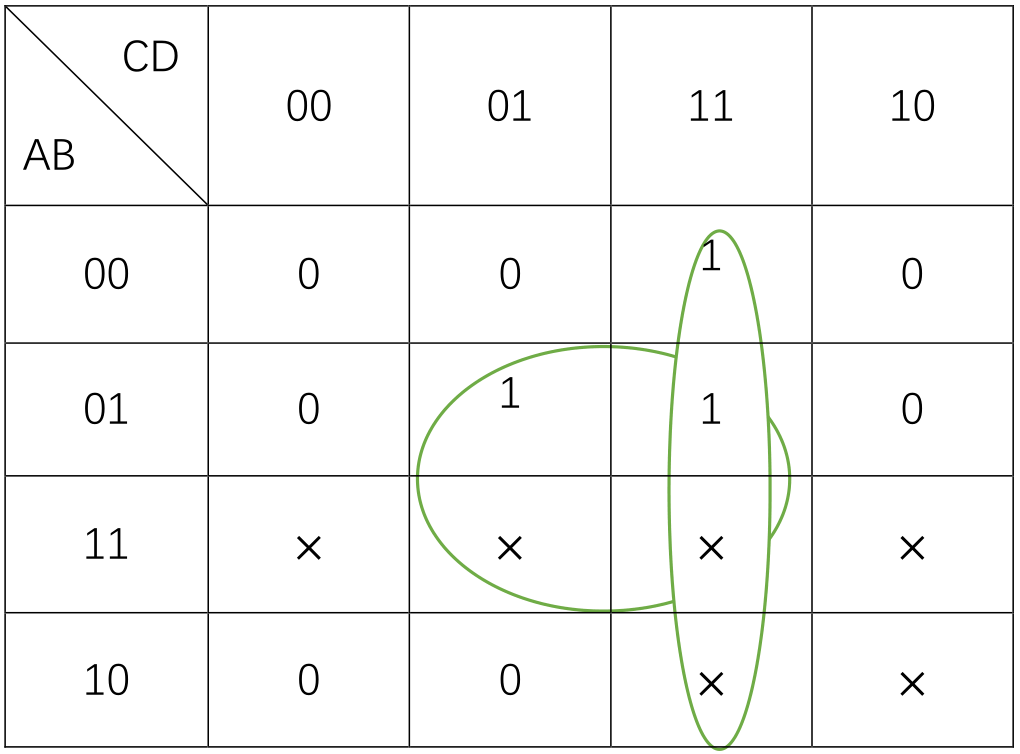
\includegraphics[width = 0.6\linewidth]{Karnaugh.png}
	\caption{卡诺图}
	\label{fig:卡诺图}
\end{figure}

根据卡诺图\ref{fig:卡诺图},分位$ 3Q_\mathrm{a}, 3Q_\mathrm{d} $和秒十位$
2Q_\mathrm{a}, 2Q_\mathrm{c} $需要连接四输入与门,当同时满足与门条件时,接入的节
点为高电平。可得到电路图如图 \ref{fig:报时电路} :

\begin{figure}[htbp]
	\centering
	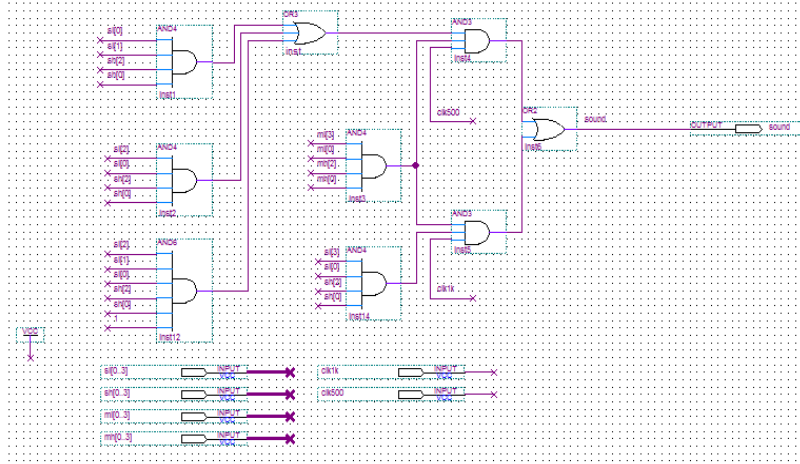
\includegraphics[width = 0.7\linewidth]{give-time.png}
	\caption{报时电路}
	\label{fig:报时电路}
\end{figure}

\subsection{秒表电路}%
\label{sub:秒表电路}

秒表电路如图\ref{fig:秒表电路}所示,实质上秒表电路内部是一个分频电路,当按下开关
后自动进行计时。精度是百分之一秒。

\begin{figure}[htbp]
	\centering
	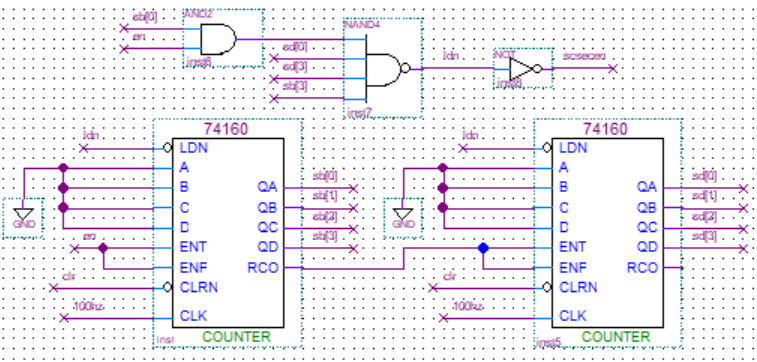
\includegraphics[width = 0.7\linewidth]{timer.png}
	\caption{秒表电路}
	\label{fig:秒表电路}
\end{figure}

\subsection{闹钟电路}%
\label{sub:闹钟电路}

当输入闹钟信号时,可以令数码管显示为闹钟数据的时间,并将闹钟时间不断赋值给闹钟时
间记录数据。否则为正常计时数据且不对闹钟时间记录数据赋值。每一个时钟上升沿进行判
断,判断此时时间是否与所记录闹钟时间数值一样,若一样则播放音乐声。

闹钟定时电路如图\ref{fig:闹钟定时电路}所示,与快速校时电路相仿,但是是在开关复用
后对时分进行加快速率。

\begin{figure}[htbp]
	\centering
	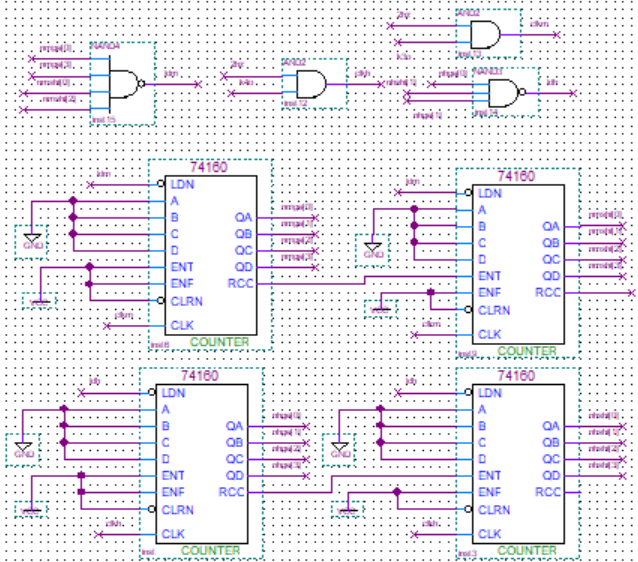
\includegraphics[width = 0.8\linewidth]{determine.png}
	\caption{闹钟定时电路}
	\label{fig:闹钟定时电路}
\end{figure}

闹钟比较电路如图\ref{fig:闹钟比较电路}所示,判断时间是否与设定时间相同。相同则播
放音乐声。

\begin{figure}[htbp]
	\centering
	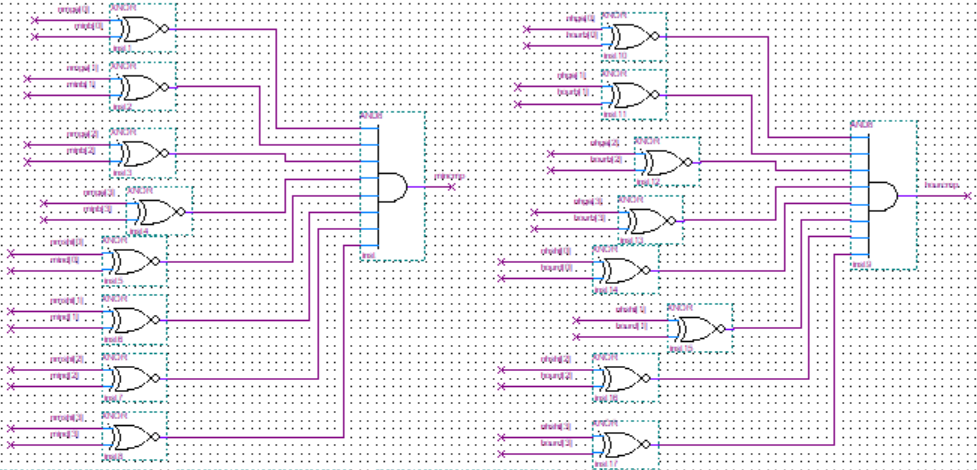
\includegraphics[width = 0.9\linewidth]{alarm.png}
	\caption{闹钟比较电路}
	\label{fig:闹钟比较电路}
\end{figure}

另外,误打误撞下意外实现了开机音乐的功能,因为闹铃在一开始没有设定时间时默认为
0点,而所以开机之后就会触发闹铃,响起音乐声。

\subsection{彩铃电路}%
\label{sub:彩铃电路}

至于闹铃使用的音乐声,本质上就是不同频率的声音。要让蜂鸣器发出不同音调的声音,就
需要用不同频率的脉冲信号去驱动蜂鸣器。表\ref{tab:音调}反映了理想情况下音调和蜂鸣
器频率的关系。

\begin{table}[htbp]
	\centering
	\caption{音调}
	\label{tab:音调}
	\csvautobooktabular{tab/music.csv}
\end{table}

对一些比较难整除的频率近似计算后,可以依据表\ref{tab:音调},搭建音调电路如图
\ref{fig:do音调电路}、 \ref{fig:re音调电路}、\ref{fig:mi音调电路}、
\ref{fig:fa音调电路}、 \ref{fig:so音调电路}、\ref{fig:la音调电路}、
\ref{fig:si音调电路}。\footnote{这样其实很繁琐,用HDL 实现会更简单。}

\begin{figure}[htbp]
	\centering
	\begin{subfigure}[htbp]{.45\linewidth}
		\centering
		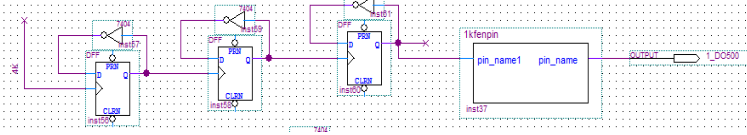
\includegraphics[width = \linewidth]{do.png}
		\caption{do音调电路}
		\label{fig:do音调电路}
	\end{subfigure}
	\quad
	\begin{subfigure}[htbp]{.45\linewidth}
		\centering
		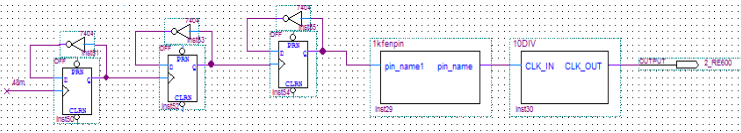
\includegraphics[width = \linewidth]{re.png}
		\caption{re音调电路}
		\label{fig:re音调电路}
	\end{subfigure}
	\quad
	\begin{subfigure}[htbp]{.45\linewidth}
		\centering
		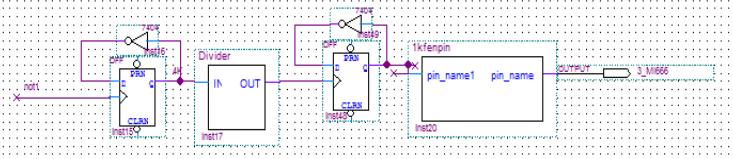
\includegraphics[width = \linewidth]{mi.png}
		\caption{mi音调电路}
		\label{fig:mi音调电路}
	\end{subfigure}
	\quad
	\begin{subfigure}[htbp]{.45\linewidth}
		\centering
		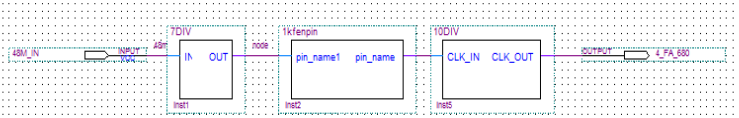
\includegraphics[width = \linewidth]{fa.png}
		\caption{fa音调电路}
		\label{fig:fa音调电路}
	\end{subfigure}
	\quad
	\begin{subfigure}[htbp]{.45\linewidth}
		\centering
		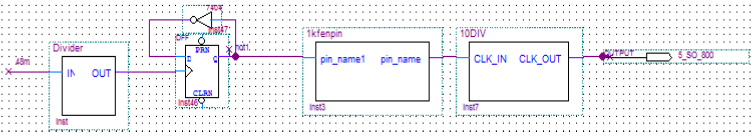
\includegraphics[width = \linewidth]{so.png}
		\caption{so音调电路}
		\label{fig:so音调电路}
	\end{subfigure}
	\quad
	\begin{subfigure}[htbp]{.45\linewidth}
		\centering
		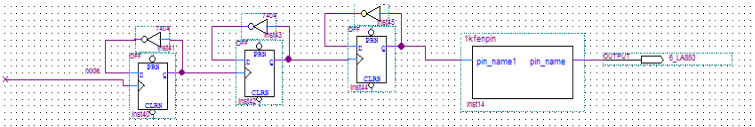
\includegraphics[width = \linewidth]{la.png}
		\caption{la音调电路}
		\label{fig:la音调电路}
	\end{subfigure}
	\quad
	\begin{subfigure}[htbp]{.45\linewidth}
		\centering
		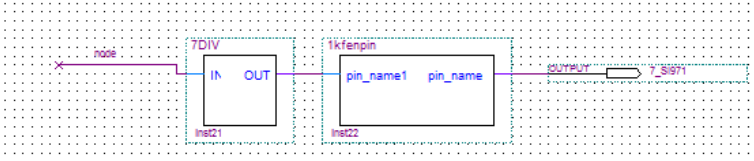
\includegraphics[width = \linewidth]{si.png}
		\caption{si音调电路}
		\label{fig:si音调电路}
	\end{subfigure}
	\begin{subfigure}[htbp]{.45\linewidth}
		\centering
		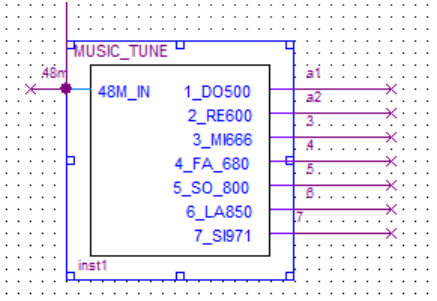
\includegraphics[width = \linewidth]{tune.png}
		\caption{音调电路}
		\label{fig:音调电路}
	\end{subfigure}
	\caption{音调}
	\label{fig:音调}
\end{figure}

如图\ref{fig:彩铃电路},歌曲采用四位 16 进制计数器 74163 进行状态计数,4-16 线译
码器 74154 对各状态依次选通,音调切换频率为\SI{1}{\Hz},能够使各声调依次响起,达
到播放音乐的功能。

\begin{figure}[htbp]
	\centering
	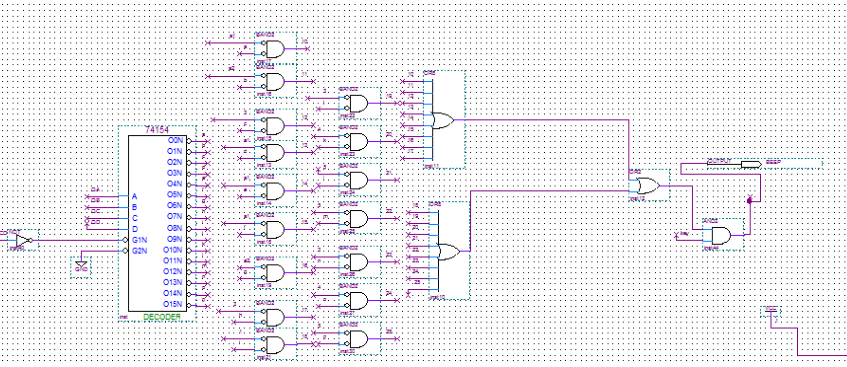
\includegraphics[width = \linewidth]{music.png}
	\caption{彩铃电路}
	\label{fig:彩铃电路}
\end{figure}

\newpage

歌曲选择如下:

\begin{score}
	%&"main"
% Fakesection 检错
% Fakesubsubsection 宏包
\RequirePackage[l2tabu, orthodox]{nag}
% Fakesubsubsection 编译器
\RequirePackage{ifxetex}
\RequireXeTeX

\documentclass[twoside, openright]{article}
% Fakesection 基础
% Fakesubsection 文字
% Fakesubsubsection 颜色
\usepackage[x11names]{xcolor}
% XXX: conflict with microtype <02-11-19> %
% Fakesubsubsection 长度
\usepackage{printlen}
\uselengthunit{mm}
% Fakesubsubsection 效果
\usepackage{ulem}
% Fakesubsubsection 字体
\usepackage{fontspec}
\setmainfont{Times New Roman}
% XXX: load ctex before siunitx to avoid \ohm ineffective <04-10-19> %
\usepackage[
	UTF8,
	fontset = windows,
	heading = true,
	zihao = -4,
	sub4section,
]{ctex}
\setCJKfamilyfont{zhsong}[
	AutoFakeBold = 2.17,
	AutoFakeSlant = 0.5,
]{SimSun}
\renewcommand*{\songti}{\CJKfamily{zhsong}}
% XXX: load newtxtext before textcomp to avoid option clash <04-10-19> %
\usepackage{newtxtext}
% Fakesubsubsection 字符边框
\usepackage{varwidth}
% Fakesubsection 断行
\usepackage{fvextra}
% Fakesubsection 标点
% XXX: load csquotes after fvextra to avoid warning <04-10-19> %
\usepackage{csquotes}
% Fakesubsubsection Unicode引号样式
\DeclareQuoteStyle{ucstyle}% style name
{\symbol{"201C}}% opening outer mark
{\symbol{"201D}}% closing outer mark
{\symbol{"2018}}% opening inner mark
{\symbol{"2019}}% closing inner mark
% Fakesubsubsection 传统中文样式
\DeclareQuoteStyle{cnzhstyle}% style name
{\symbol{"300E}}% opening outer mark
{\symbol{"300F}}% closing outer mark
{\symbol{"300C}}% opening inner mark
{\symbol{"300D}}% closing inner mark
\setquotestyle{cnzhstyle}
% Fakesubsubsection 书名号样式
\DeclareQuoteStyle{zhtitlestyle}% style name
{\symbol{"300A}}% opening outer mark
{\symbol{"300B}}% closing outer mark
{\symbol{"3008}}% opening inner mark
{\symbol{"3009}}% closing inner mark
% Fakesubsection 样式
% Fakesubsubsection 目录
\usepackage{titletoc}
\titlecontents{section}[0pt]{\filright}{\contentspush{\thecontentslabel}}{}{\titlerule*{.}\contentspage}
% Fakesubsubsection 章节
\ctexset{
	section = {
		name = ,
		number = \arabic{section},
		aftername = \hspace{1\ccwd},
		format = \ifthenelse{\value{section}=0}{\centering}{}\zihao{3}\heiti\bfseries,
		beforeskip = 0.5\ccwd,
		afterskip = 0.5\ccwd,
	},
	subsection = {
		aftername = \hspace{1\ccwd},
		format = \ifthenelse{\value{section}=0}{\centering}{}\zihao{-3}\heiti\bfseries,
		beforeskip = 0.5\ccwd,
		afterskip = 0.5\ccwd,
	},
	subsubsection = {
		format = \zihao{4}\heiti\bfseries,
	}
}
% Fakesubsubsection 图表
\usepackage{caption}
\captionsetup[figure]{labelsep=space}
\captionsetup[table]{labelsep=space}
\captionsetup{font=small}
\DeclareCaptionFont{blue}{\color{LightSteelBlue3}}
\setlength{\abovecaptionskip}{0.5\ccwd}
\setlength{\belowcaptionskip}{0.5\ccwd}
% Fakesubsubsection 子图表
\usepackage{subcaption}
% Fakesubsubsection 公式
\setlength{\abovedisplayskip}{0.5em}
\setlength{\belowdisplayskip}{0.5em}
% Fakesubsubsection 列表
\usepackage{enumitem}
\setlist[enumerate, 1]{
	fullwidth,
	label = (\arabic*),
	font = \textup,
	itemindent=2em
}
\setlist[enumerate, 2]{
	fullwidth,
	label = (\alph*),
	font = \textup,
	itemindent=4em
}
% Fakesubsubsection 代码
% XXX: need -shell-escape & pygmentize <04-10-19> %
\usepackage{minted}
\usepackage{boxie}
% XXX: conflict with fancybox <02-11-19> %
% Fakesubsubsection 问答
\usepackage{exercise}
\usepackage{tasks}
% Fakesubsubsection 改动

% Fakesection 插入
% Fakesubsection 表格
% Fakesubsubsection 三线
\usepackage{booktabs}
% Fakesubsubsection 对角线
\usepackage{diagbox}
% Fakesubsubsection 合并列
\usepackage{multicol}
% Fakesubsubsection 合并行
\usepackage{multirow}
% Fakesubsubsection 分割单元格
\usepackage{makecell}
% Fakesubsubsection 短表
\usepackage{tabu}
% Fakesubsubsection 长表
\usepackage{longtable}
% Fakesubsubsection 彩色表
\usepackage{colortbl}
\usepackage{tcolorbox}
\tcbuselibrary{skins}
\tcbuselibrary{breakable}
\tcbuselibrary{theorems}
\tcbuselibrary{listings}
\tcbuselibrary{xparse}
% XXX: need -shell-escape & pygmentize <04-10-19> %
\tcbuselibrary{minted}
% Fakesubsubsection 导入数据
\usepackage{csvsimple}
% Fakesubsection 图形
% Fakesubsubsection 插图
\usepackage{graphicx}
\graphicspath{{fig/}{etc/}}
% Fakesubsubsection 环绕
\usepackage{wrapfig}
% Fakesubsubsection 图片重叠
\usepackage{overpic}
% Fakesubsubsection 徽标
\usepackage{hologo}
% Fakesubsubsection 条形码
\usepackage{ean13isbn}
% Fakesubsubsection 二维码
\usepackage{qrcode}
% Fakesubsection 符号
% Fakesubsubsection 数学符号
\usepackage{newtxmath}
\usepackage{bm}
% Fakesubsubsection 幻灯片符号
\usepackage{pifont}
% Fakesubsubsection 大数学符号
\usepackage{exscale}
% Fakesubsubsection 数学符号放缩
\usepackage{relsize}
% Fakesubsubsection 公式
\usepackage{cases}
\usepackage{physics}
% Fakesubsubsection 单位
\usepackage{siunitx}
\sisetup{mode=text}
% Fakesubsubsection 计算机
% Fakesubsubsection 音乐
\usepackage{mtxlatex}
\mtxlatex
% Fakesubsection 媒体
\usepackage{media9}
% Fakesubsection 链接
\usepackage[
	colorlinks = true,
	linkcolor = gray,
	citecolor = gray,
	backref = page
]{hyperref}
% Fakesubsection 批注
\usepackage{todonotes}
\usepackage{cooltooltips}
\usepackage{pdfcomment}
% Fakesubsection 文本框
\usepackage{boxedminipage2e}
% Fakesubsection 页眉页脚
\usepackage{fancyhdr}
\fancypagestyle{plain}{
	\pagestyle{fancy}
}

% Fakesection 设计
% Fakesubsection 水印
\usepackage{wallpaper}
% Fakesubsection 主题

% Fakesection 布局
% Fakesubsection 页面
\usepackage{geometry}
% Fakesubsection 缩进
\usepackage{indentfirst}
% Fakesubsection 间距
\usepackage{setspace}
\usepackage[
	restoremathleading=false,
	UseMSWordMultipleLineSpacing,
	MSWordLineSpacingMultiple=1.5
]{zhlineskip}
% Fakesection 引用
% Fakesubsection 脚注
\renewcommand{\thefootnote}{\fnsymbol{footnote}}
\renewcommand{\thempfootnote}{\fnsymbol{mpfootnote}}
% Fakesubsection 引文
\usepackage{morewrites}
\usepackage[square, comma, numbers, super, sort&compress, longnamesfirst, sectionbib, nonamebreak]{natbib}
% Fakesubsection 题注
\usepackage{epigraph}
% Fakesubsection 索引
\usepackage{makeidx}
\makeindex
% Fakesubsection 关联
% XXX: need amsmath <04-10-19> %
%\numberwithin{Exercise}{chapter}
%\numberwithin{Answer}{chapter}

% Fakesection 特殊功能
% Fakesubsection 页数统计
\usepackage{lastpage}
% Fakesubsection 数学表达式
\usepackage{calc}

\begin{document}

% Fakesection 扉页

\newcommand{\Title}{EDA设计实验报告}

\begin{titlepage}
	\centering
	\begin{spacing}{1}
		\zihao{4}
		\vspace{0.5\ccwd}

		\vspace{1\ccwd}

		\includegraphics[width=7.41cm]{NJUST.ai}

		\vspace{0.2\ccwd}

		\fontsize{45pt}{45pt}\selectfont\heiti
		\Title

		\zihao{-1}
		\vspace{2\ccwd}
	\end{spacing}

	\begin{spacing}{1.5}
		\zihao{3}
		\begin{tabu} to 12.59cm{@{}X[c, 3.2cm]@{}X[c, 4cm]@{}X[c, 2.22cm]@{}X[c, 3.89cm]@{}}
			\textbf{作  者:} & \underline{\makebox[4cm][c]{\kaishu 吴振宇}} & \textbf{学 号:} & \underline{\makebox[3.89cm][c]{\kaishu 916101630117}} \\
			\textbf{学  院:} & \multicolumn{3}{c}{\underline{\makebox[10.11cm][c]{\kaishu 电子工程与光电技术学院}}} \\
			\textbf{专业(方向):} & \multicolumn{3}{c}{\underline{\makebox[10.11cm][c]{\kaishu 电子信息工程}}} \\
			\textbf{班  级:} & \multicolumn{3}{c}{\underline{\makebox[10.11cm][c]{\kaishu 电信4班}}} \\
			\textbf{题  目:} & \multicolumn{3}{c}{\underline{\makebox[10.11cm][c]{\kaishu 多功能数字时钟设计}}} \\
			\textbf{} & \multicolumn{3}{c}{\underline{\makebox[10.11cm][c]{\kaishu}}}
		\end{tabu}
		\vspace{0em}
	\end{spacing}

	\begin{spacing}{1}
		\zihao{3}
		\vspace{3\ccwd}

		\zihao{-3}
		\textbf{指导者:}\underline{\makebox[15.5\ccwd][c]{}}

		\zihao{5}
		\hspace{5em}(姓名)\hspace{11em}(专业技术职务)

		\zihao{-3}
		    \underline{\makebox[15.5\ccwd][c]{}}

		\zihao{5}
		\hspace{5em}(姓名)\hspace{11em}(专业技术职务)

		\zihao{-3}
		\textbf{评阅者:}\underline{\makebox[15.5\ccwd][c]{}}

		\zihao{5}
		\hspace{5em}(姓名)\hspace{11em}(专业技术职务)

		\zihao{3}
		\vspace{2\ccwd}

		\zihao{-2}
		\number\year 年\number\month 月
	\end{spacing}
	\vspace{0em}
\end{titlepage}

% Fakesection 声明

\renewcommand{\abstractname}{\zihao{3}\heiti 声\hspace{2\ccwd}明}
\begin{abstract}
	\zihao{4}

	我声明,本\Title 及其研究工作和所取得的成果是本人在导师的指导下独立完成
	的。研究过程中利用的所有资料均已在参考文献中列出,其他人员或机构对本
	\Title 工作做出的贡献也已在致谢部分说明。

	本\Title 不涉及任何秘密,南京理工大学有权保存其电子和纸质文档,可以借阅
	或网上公布其部分或全部内容,可以向有关部门或机构送交并授权保存、借阅或网
	上公布其部分或全部内容。

	\vspace{2\ccwd}

	\begin{flushright}
		学生签名:\hspace{8em}

		\vspace{1\ccwd}

		年\hspace{3em}月\hspace{3em}日

		\vspace{2\ccwd}

		指导教师签名:\hspace{8em}

		\vspace{1\ccwd}

		年\hspace{3em}月\hspace{3em}日
	\end{flushright}
\end{abstract}

% Fakesection 摘要页眉页脚

\pagestyle{fancy}
\renewcommand{\headrulewidth}{0pt}
\fancyhead[LC, RC]{}
\fancyhead[LE, RO]{}
\fancyhead[RE, LO]{}
\fancyfoot[LC, RC]{}
\fancyfoot[LE, RO]{}
\fancyfoot[RE, LO]{}

% Fakesection 摘要

\newpage

\begin{center}
	\zihao{3}\renewcommand{\CJKglue}{\hskip 2pt}\heiti \Title 中文摘要

	\vspace{0.3em}

	\begin{boxedminipage}[][18cm]{\linewidth}
		\begin{spacing}{1.5}
			\zihao{-4}

			\vspace{1\ccwd}

			本实验利用 QuartusII 软件设计一个多功能数字计时器,并下
			载到 SmartSOPC 实验系统中。这个数字计时器,可以完成
			00:00:00 到 23:59:59 的计时功能,并在控制电路的作用下具
			有保持、清零、快速校时、快速校分、整点报时等功能,这些
			功能相互独立,却又互相协调配合。在此类基础功能之上还添
			加了显示星期、闹钟、秒表、彩铃功能。
			\cite{姜萍2008创新教育在, 2010数字逻辑电路基础, 孙敦艳2011硬件描述语言在数字逻辑电路教学中的应用}

			\vspace{2\ccwd}

			\noindent\textbf{关键词}\hspace{1\ccwd}多功能数字钟\hspace{1\ccwd}SmartSOPC\hspace{1\ccwd}QuartusII
		\end{spacing}
	\end{boxedminipage}
\end{center}

% Fakesection 英文摘要

\newpage

\begin{center}
	\zihao{3}\renewcommand{\CJKglue}{\hskip 2pt}\heiti \Title 英文摘要

	\vspace{0.3em}

	\begin{boxedminipage}[][18cm]{\linewidth}
		\begin{spacing}{1.5}
			\zihao{3}

			\vspace{1em}

			\begin{tabu} to \linewidth{@{}X[l]@{}X[l, 8]@{}}
				\textbf{Title} & \hspace{2em}\underline{\makebox[15em][c]{\zihao{4}\songti Multi-functional Digital Timer}} \\
					       & \hspace{2em}\underline{\makebox[15em][c]{\zihao{4}\songti }} \\
			\end{tabu}

			\textbf{Abstract}

			\zihao{-4} In this experiment, QuartusII software is
			used to design a multi-functional digital timer, which
			is downloaded to the smartsopc experimental system.
			This digital timer can complete the timing function from
			00:00:00 to 23:59:59. Under the control circuit, it has
			the functions of keeping, clearing, fast time
			calibration, fast time calibration and whole time
			reporting. These functions are independent of each
			other, but coordinated with each other. In addition to
			such basic functions, has added displaying week, alarm
			clock, stopwatch and polyphonic ringtone.

			\vspace{2em}

			\noindent\textbf{Keywords}\hspace{1em}multi-functional digital timer\hspace{1em}SmartSOPC\hspace{1em}QuartusII
		\end{spacing}
	\end{boxedminipage}
\end{center}

% Fakesection 目录页眉页脚

\newpage

\renewcommand{\headrulewidth}{0.4pt}
\fancyhead[LC, RC]{\zihao{-2}\Title}
\fancyhead[LE, RO]{\zihao{5}第\thepage 页}
\fancyhead[RE, LO]{}

% Fakesection 目录

\pagenumbering{roman}

\setcounter{tocdepth}{2}

\renewcommand{\contentsname}{\zihao{3}\heiti 目次}
\tableofcontents
\listoffigures
\listoftables

\newpage
\pagenumbering{arabic}

% Fakesection 正文

\section{实验要求}%
\label{sec:实验要求}

\subsection{实验基本要求}%
\label{sub:实验基本要求}

\begin{enumerate}

	\item 能进行正常的时、分、秒计时功能;

	\item $ K_1 $是系统的使能开关($ K_1 = 0$正常工作,$ K_1 = 1$数字钟保持
		不变);

	\item $ K_2 $是系统的清零开关($ K_2 = 0$正常工作,$ K_2 = 1$数字钟全清
		零);

	\item $ K_3 $是系统的校分开关($ K_3 = 0$正常工作,$ K_3 = 1$时可以快速
		校分);

	\item $ K_4 $是系统的校时开关($ K_4 = 0$正常工作,$ K_4 = 1$时可以快速
		校时);

	\item 使数字钟具有整点报时功能(当数字钟计到\ang{;59;53}时开始报时,在
		\ang{;59;53}\ang{;59;55}\ang{;59;57}时报时频率为
		\SI{500}{\Hz};\ang{;59;59}时报时频率为\SI{1}{\kHz})。

\end{enumerate}

\subsection{实验提高要求}%
\label{sub:实验提高要求}

\begin{enumerate}

	\item 添加星期功能;

	\item 万年历功能;

	\item 闹表设定功能;

	\item 秒表功能;

	\item 自己添加其他功能;

	\item 彩铃功能。

\end{enumerate}

\section{子模块设计及原理图}%
\label{sec:子模块设计及原理图}

根据实验要求章节\ref{sec:实验要求},一共有如下6大子电路,其相互关系见图
\ref{fig:电路整体框图}。

\begin{figure}[htbp]
	\centering
	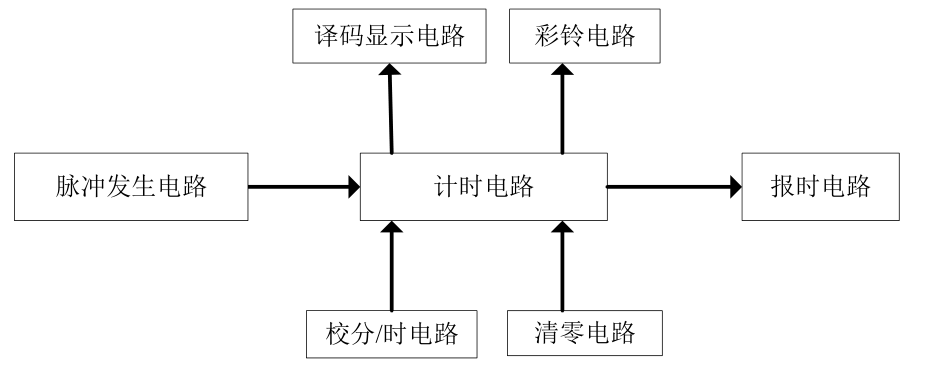
\includegraphics[width=0.8\linewidth]{block.png}
	\caption{电路整体框图}
	\label{fig:电路整体框图}
\end{figure}

按功能可进一步细分为以下部分:

\begin{description}

	\item[\nameref{sub:脉冲发生电路}:] 通过对主时钟进行分频,产生\SI{1}{\kHz},
		\SI{500}{\Hz}, \SI{2}{\Hz}, \SI{1}{\Hz}等电路所需要的时钟频率;

	\item[\nameref{sub:计时电路}:] 采用计数器组成,对\SI{1}{\Hz}信号进行计数,是整个电路的
		核心;

	\item[\nameref{sub:校分/时电路}:] 快速调整分钟/小时,以便对电路进行检测;

	\item[\nameref{sub:计数保持电路}:] 保持计数值不变;

	\item[\nameref{sub:清零电路}:] 将所有计数器清零,用以检测电路;

	\item[\nameref{sub:消抖电路}:] 接在按键输入端后,以消除抖动;

	\item[\nameref{sub:显示译码电路}:] 将计数器的输出数字翻译成数码管的显示数字,并采用
		\SI{1}{\kHz}信号使数码管动态显示;

	\item[\nameref{sub:报时电路}:] 当计数器数值达到预定值的时候,蜂鸣器响起,达到类似闹钟的
		效果;

	\item[\nameref{sub:闹钟电路}:] 开关复用后,通过定时定分设定闹铃的预定时
		间;

	\item[\nameref{sub:彩铃电路}:] 到达闹铃的预定时间,蜂鸣器的报时信号为音乐;

	\item[\nameref{sub:秒表电路}:] 显示从0开始经过的时间。

\end{description}

\subsection{脉冲发生电路}%
\label{sub:脉冲发生电路}

实验中提供稳定的频率为\SI{48}{\MHz}的高频脉冲,需使用到系统时钟\SI{1}{\Hz}、报时
电路中蜂鸣器使用的\SI{2}{\kHz}、\SI{1}{\kHz}频率,故需要将时钟信号分频。

\begin{figure}[htbp]
	\centering
	\begin{subfigure}[htbp]{.45\linewidth}
		\centering
		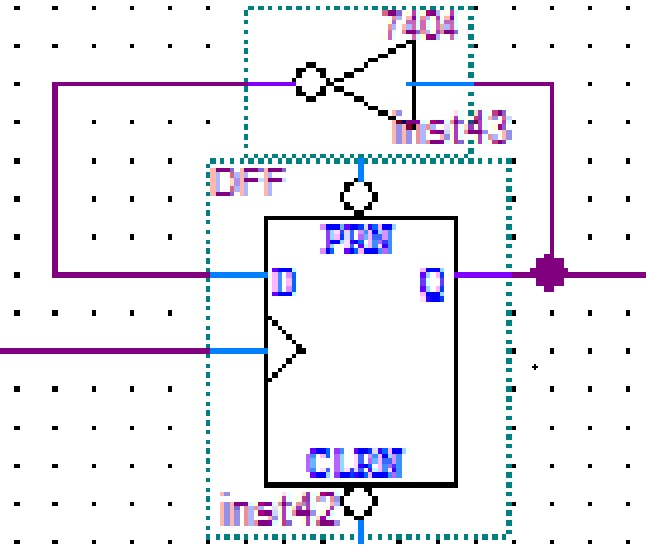
\includegraphics[width=\linewidth]{2.jpg}
		\caption{2分频}
		\label{fig:2分频}
	\end{subfigure}
	\quad
	\begin{subfigure}[htbp]{.45\linewidth}
		\centering
		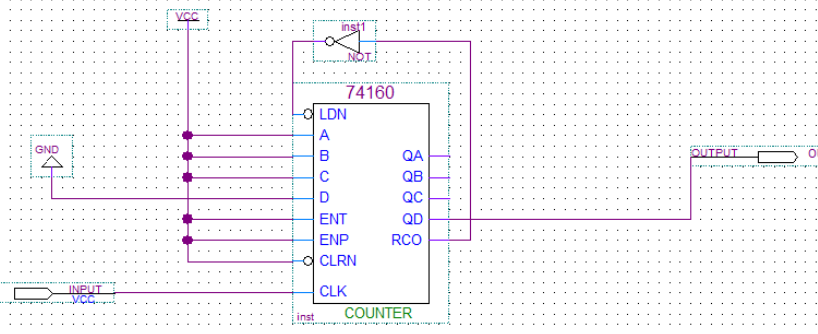
\includegraphics[width=\linewidth]{3.png}
		\caption{3分频}
		\label{fig:3分频}
	\end{subfigure}

	\begin{subfigure}[htbp]{.45\linewidth}
		\centering
		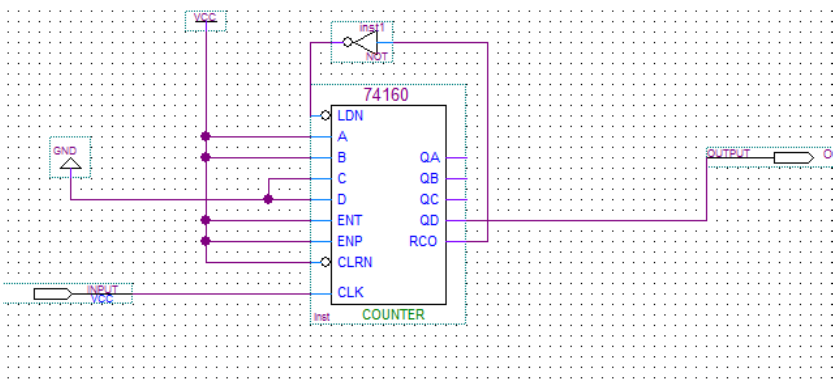
\includegraphics[width=\linewidth]{7.png}
		\caption{7分频}
		\label{fig:7分频}
	\end{subfigure}
	\quad
	\begin{subfigure}[htbp]{.45\linewidth}
		\centering
		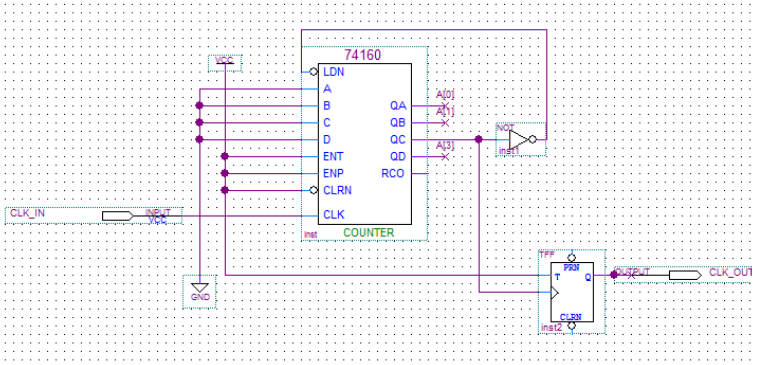
\includegraphics[width=\linewidth]{10.png}
		\caption{10分频}
		\label{fig:10分频}
	\end{subfigure}

	\caption{分频电路}
	\label{fig:分频电路}
\end{figure}

如图\ref{fig:2分频},二分频器采用一个 D 触发器和一个非门组成 T 触发器,其状态方
程为:

\begin{align}
	Q^{n + 1} = Q^n
\end{align}

每当一个上升沿到来,计数器翻转一次,可对输入信号进行二分频。

如图\ref{fig:3分频},采用模十计数器 74160 组成模 3 计数器,其有效状态有 0111,
1000,1001,当计数到 1001 时,输出端 RCO 输出信号到计数器置数端,使计数器回到状
态 0111。经过分频后的输出信号为计数值的高位。仿真波形图如图\ref{fig:3分频仿真}。

如图\ref{fig:7分频},与三分频电路类似,采用计数器 74160 和非门组成模 7 计数器,
采用置数法,其有效状态共 7 种:0011,0100,0101,0110,0111,1000,1001。当电路计数到
1001 时,RCO 端发出置数信号,使计数器回到初始状态。由最高位 QD 取出信号,得到经
过 7 分频之后的时钟信号。仿真波形图如图\ref{fig:7分频仿真}。七分频电路方便进行星
期的显示。

如图\ref{fig:10分频},采用模十计数器 74160 构成模 5 计数器,再添加一个 T 触发器
构成二分频器便得到了 10 分频器,其有效状态有:0000,0001,0010,0011,0100。仿真波形
图如图\ref{fig:10分频仿真}。

\begin{figure}[htbp]
	\centering
	\begin{subfigure}[htbp]{.31\linewidth}
		\centering
		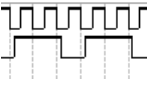
\includegraphics[width = \linewidth]{3-2.png}
		\caption{3分频仿真}
		\label{fig:3分频仿真}
	\end{subfigure}
	\quad
	\begin{subfigure}[htbp]{.31\linewidth}
		\centering
		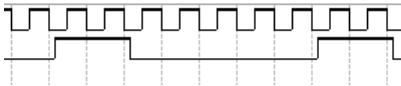
\includegraphics[width = \linewidth]{7-2.png}
		\caption{7分频仿真}
		\label{fig:7分频仿真}
	\end{subfigure}
	\quad
	\begin{subfigure}[htbp]{.31\linewidth}
		\centering
		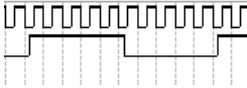
\includegraphics[width = \linewidth]{10-2.png}
		\caption{10分频仿真}
		\label{fig:10分频仿真}
	\end{subfigure}
	\caption{分频仿真}
	\label{fig:分频仿真}
\end{figure}

总的原理图如图\ref{fig:分频原理图}。

\begin{figure}[htbp]
	\centering
	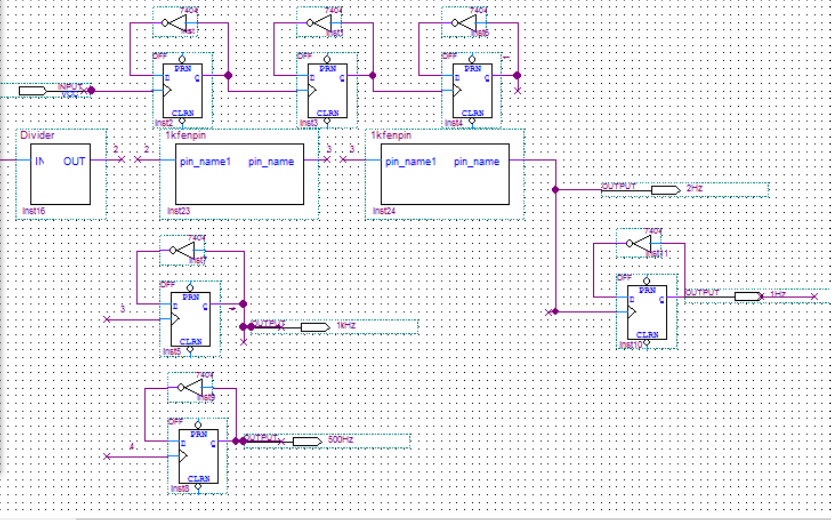
\includegraphics[width = 0.8\linewidth]{divider.png}
	\caption{分频原理图}
	\label{fig:分频原理图}
\end{figure}

可以看到用原理图搭建电路繁琐麻烦。可以考虑使用硬件描述语言对电路进行行为级建模。
思路为:对时钟信号进行上升沿检测,并记录检测的数(从 0 开始计数)。如果是$ N $分
频,每当计数到$ \dfrac{N}{2} - 1 $时将信号翻转一次,将信号输出。

\langCVfile[verilog][lst:divider.v][verilog]{divider.v}{lst/divider.v}

\langCVfile[verilog][lst:divider.vt][verilog]{divider.vt}{lst/divider.vt}

\subsection{计时电路}%
\label{sub:计时电路}

如图\ref{fig:计时电路}所示,秒个位在输入时钟信号上升沿时进行计数,其值从0000到
1001循环。在计时过程中,当秒个位的状态由1001变为0000时,秒十位接收一个进位信号来
实现进位,该信号为秒个位的下降沿(由“1”到“0”的变化),从而实现进位。同理可得秒十
位向分个位的进位信号。

\begin{figure}[htbp]
	\centering
	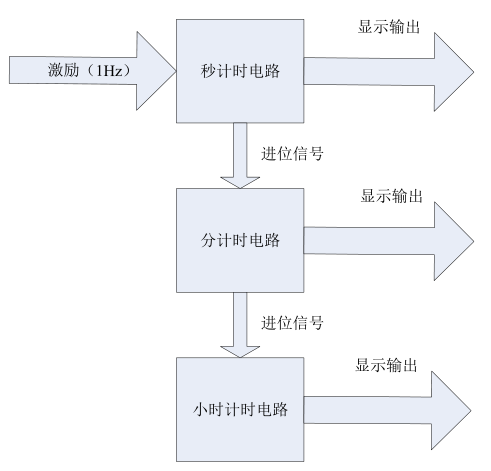
\includegraphics[width = 0.6\linewidth]{count.png}
	\caption{计时电路}
	\label{fig:计时电路}
\end{figure}

秒计数器的模为 60,电路上采用十进制计数器 74160 构成一个模 10 计数器和一个模 6
计数器,再将两者接在同一计数脉冲上,可得到模 60 计数器。

\begin{figure}[htbp]
	\centering
	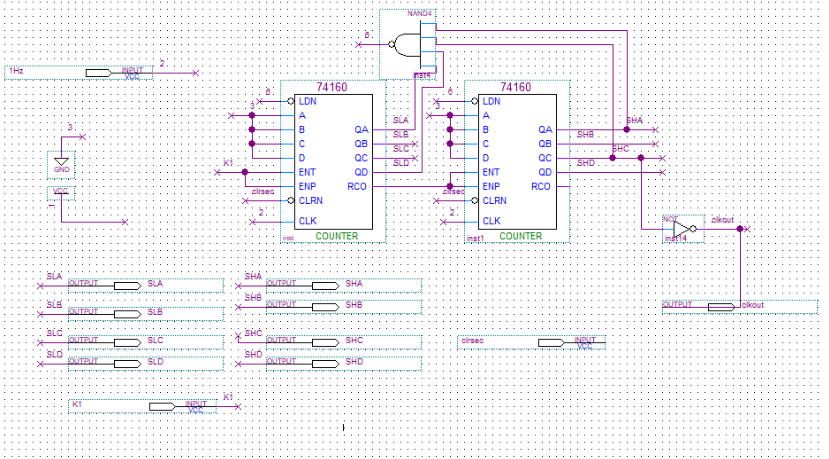
\includegraphics[width = 0.8\linewidth]{sec.png}
	\caption{秒/分计时电路}
	\label{fig:秒/分计时电路}
\end{figure}

\begin{figure}[htbp]
	\centering
	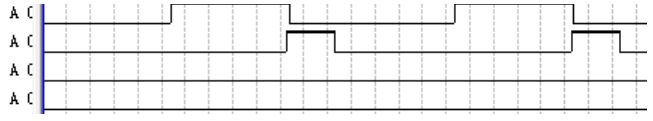
\includegraphics[width = 0.8\linewidth]{sec-1.png}
	\caption{秒/分计时电路低位仿真波形}
	\label{fig:秒/分计时电路低位仿真波形}
\end{figure}

\begin{figure}[htbp]
	\centering
	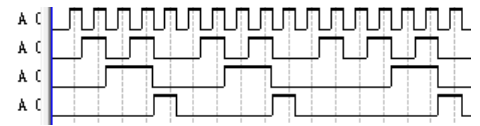
\includegraphics[width = 0.8\linewidth]{sec-2.png}
	\caption{秒/分计时电路高位仿真波形}
	\label{fig:秒/分计时电路高位仿真波形}
\end{figure}

如图\ref{fig:秒/分计时电路} 所示,左边计数器为低位的模十计数器,每来一个脉冲计数
值加一,其计数状态为 0 到 9 。低位计数器的 RCO 端接到高位计数器的 ENT、ENP,低位
计数值为 0 到 8 时,高位计数器停止计数。当低位计数器计数值为 9 时,RCO 端输出变
为高电平,高位计数器被使能,当下一个脉冲到来时,高位加一计数,达到计数进位的功能
,而此时低位由最大值变为最小值。

当清零输入端接入逻辑 0 时,电路计数值被清零;$ K_1 $为计数保持端,当该端口接入逻
辑 0 的时候,计数器保持当前数值,且忽略输入的脉冲信号。右方各端口分别表示秒高位
和低位的四个计数端 A、B、C、D,可接入动态显示用。

图\ref{fig:秒/分计时电路低位仿真波形}中秒计数的低位仿真波形状态为:0000 0001
0010 0011 0100 0101 0110 0111 1000 1001,为十进制的 0 到 9 共计 10 个状态。图
\ref{fig:秒/分计时电路高位仿真波形}中秒计数高位的仿真波形状态为:0000 0001 0010
0011 0100 0101 ,为十进制的 0 到 5,共计 6 个状态。可见,该电路满足模为 60 的秒
计数电路。分计数电路与秒计数电路同理。

\begin{figure}[htbp]
	\centering
	\includegraphics[width = 0.8\linewidth]{min.png}
	\caption{时计时电路}
	\label{fig:时计时电路}
\end{figure}

\begin{figure}[htbp]
	\centering
	\includegraphics[width = 0.8\linewidth]{min-1.png}
	\caption{时计时电路低位仿真波形}
	\label{fig:时计时电路低位仿真波形}
\end{figure}

\begin{figure}[htbp]
	\centering
	\includegraphics[width = 0.8\linewidth]{min-2.png}
	\caption{时计时电路高位仿真波形}
	\label{fig:时计时电路高位仿真波形}
\end{figure}

时计数器为模 24 。电路上采用两个模十计数器 74160 构成。当小时的高位为 0 或 1 两
种情况时,小时的低位按模 10 计数,有效状态为从 0 到 9 ;当小时的高位为 2 时,小
时的低位按模 4 计数,有效状态为从 0 到 3;由图\ref{fig:时计时电路}可知,同步置数
端信号有效的条件是:低位计数值为 0011 ,高位计数值为 0010,即计数器计数到 23 时
,下一个脉冲的上升沿使两个计数器回到 0000 的状态,达到模 24 计数的功能。

时计数器除了接小时位的清零开关、分钟计数的进位信号、小时的保持开关和小时快速计数
的输入脉冲外,小时高位和低位的 4 个计数位 A B C D 可接入动态显示端口用以动态显示
。图\ref{fig:时计时电路低位仿真波形}为小时计数电路的个位仿真波形图,可见在前两个
周期,其计数状态由 0000 到 1001 ,为十进制的 0 到 9。 在第三个周期,其计数状态变
为从 0000 到 0011 ,为十进制的 0 到 3 ;对于图 \ref{fig:时计时电路高位仿真波形}
为小时计数的十位仿真波形图,其计数状态为 0000 到 0010,为十进制的 0 到 2。满足小
时计数的要求。

\subsection{校分/时电路}%
\label{sub:校分/时电路}

实现校准时,校准信号为1,此时,若校秒信号为1,则秒个位输入时钟应该为\SI{1}{\Hz}信
号以进行校秒,若快速校秒信号为1,则秒个位输入时钟应该为\SI{2}{\Hz}信号以进行快速
校秒。

\begin{figure}[htbp]
	\centering
	\includegraphics[width = 0.8\linewidth]{calibrate.png}
	\caption{校准电路}
	\label{fig:校准电路}
\end{figure}

图\ref{fig:校准电路}所示是校分(校时)电路原理图。当开关拨下时,分计数器和小时计
数器的输入频率被切换到\SI{2}{\Hz},原计数进位信号被屏蔽,从而实现快速校分(校时
)的功能。当开关拨回原位置的时候,电路的输入脉冲回到\SI{1}{\Hz}的正常计数模式,
其中秒位不设快速计数功能。如图所示,$ K_4 $端是校分(校时)的开关端口,当$ K_4 =
1 $时,与\SI{2}{\Hz}的输入频率相与,经过或门,\SI{2}{\Hz}信号给入计数器的时钟端
口,当$ K_4 = 0 $时,\SI{2}{\Hz}的输入经与门被置零,$ K_4 $经过非门,与秒计数器
或分计数器的进位端相与,之后经过或门送入分(时)计数器的时钟端,从而在$ K_4 = 0
$ 时正常计数。

\subsection{计数保持电路}%
\label{sub:计数保持电路}

\begin{wrapfigure}{r}{0.6\linewidth}
	\centering
	\includegraphics[width = \linewidth]{keep.png}
	\caption{计数保持电路}
	\label{fig:计数保持电路}
	\vspace{-4em}
\end{wrapfigure}

如图\ref{fig:计数保持电路}所示,保持电路的实现依赖于计数器本身的保持端口 ENT、
ENP,当保持端接 1 时,计数器正常计数;当保持端接 0 时,计数器会忽略时钟端口到来
的脉冲信号,保持现有的数值不变。同清零电路一样,保持电路也有消抖电路作为中间缓冲
区消除机械抖动。

\subsection{清零电路}%
\label{sub:清零电路}

如图\ref{fig:清零电路}所示,清零电路是在任何状态下将电路归零的电路,由$ U_4 $控
制,$ U_4 = 1 $时,各个位的数字置0 。

\begin{figure}[htbp]
	\centering
	\includegraphics[width = 0.6\linewidth]{clear.png}
	\caption{清零电路}
	\label{fig:清零电路}
\end{figure}

\subsection{消抖电路}%
\label{sub:消抖电路}

如图\ref{fig:消抖电路}所示,将开关连接到 D 触发器的输入端。以清零开关为例,当开
关处于拨下状态时,计数器清零端有效,计时器数值清零。而在开关拨下的过程中,由于机
械抖动,开关输入到计数器的信号是不稳定的,将会导致计数器的数值不断乱跳。将其接入
D 触发器后,颤抖明显被消除,输入信号稳定性得到改善。

\begin{figure}[htbp]
	\centering
	\includegraphics[width = 0.6\linewidth]{tremble.png}
	\caption{消抖电路}
	\label{fig:消抖电路}
\end{figure}

\subsection{显示译码电路}%
\label{sub:显示译码电路}

动态扫描是把所有显示器的8个段码中的a-dp的各个相同段连接在一起, 接到一个公共的输
出口上,而数码管的位端分别接在另外的输出口上,通过这两个输出口的两组信号相互作用
来产生显示效果。即让各位数码管按照一定顺序轮流显示, 只要扫描频率足够高, 由于人
眼的“视觉暂留”现象,就能连续稳定的显示。本次实验中选择了\SI{1}{\kHz}。

\begin{figure}[htbp]
	\centering
	\includegraphics[width = 0.8\linewidth]{display.png}
	\caption{显示译码电路}
	\label{fig:显示译码电路}
\end{figure}

按照高电平对应的数码管被点亮的工作方式, 该数码管为阳极驱动。如图
\ref{fig:显示译码电路},四个 8 选 1 数据选择器 74151 一起组成了 24 选 4 数据选择
器(每个数据选择器只使用了 6 位),将 6 个数字轮流送到数码管译码器 7474 进行译码
显示。74138 为译码器,用于点亮数字所对应的数码管。输入\SI{1}{\kHz}的刷新频率用于
动态显示。

\subsection{报时电路}%
\label{sub:报时电路}

报时电路要求在每个小时里,分钟位和秒位计数达到 59 分 53 秒,59 分 55 秒,59 分
57 秒时,蜂鸣器输出低频信号声音,在 59 分 59 秒蜂鸣器输出高频信号声音。将四种情
况列于表\ref{tab:报时电路}:

\begin{table}[htbp]
	\centering
	\caption{报时电路}
	\label{tab:报时电路}
	\csvautobooktabular{tab/give-time.csv}
\end{table}

画出卡诺图如图\ref{fig:卡诺图}\footnote{X表示其中的无效状态}。

\begin{figure}[htbp]
	\centering
	\includegraphics[width = 0.6\linewidth]{Karnaugh.png}
	\caption{卡诺图}
	\label{fig:卡诺图}
\end{figure}

根据卡诺图\ref{fig:卡诺图},分位$ 3Q_\mathrm{a}, 3Q_\mathrm{d} $和秒十位$
2Q_\mathrm{a}, 2Q_\mathrm{c} $需要连接四输入与门,当同时满足与门条件时,接入的节
点为高电平。可得到电路图如图 \ref{fig:报时电路} :

\begin{figure}[htbp]
	\centering
	\includegraphics[width = 0.7\linewidth]{give-time.png}
	\caption{报时电路}
	\label{fig:报时电路}
\end{figure}

\subsection{秒表电路}%
\label{sub:秒表电路}

秒表电路如图\ref{fig:秒表电路}所示,实质上秒表电路内部是一个分频电路,当按下开关
后自动进行计时。精度是百分之一秒。

\begin{figure}[htbp]
	\centering
	\includegraphics[width = 0.7\linewidth]{timer.png}
	\caption{秒表电路}
	\label{fig:秒表电路}
\end{figure}

\subsection{闹钟电路}%
\label{sub:闹钟电路}

当输入闹钟信号时,可以令数码管显示为闹钟数据的时间,并将闹钟时间不断赋值给闹钟时
间记录数据。否则为正常计时数据且不对闹钟时间记录数据赋值。每一个时钟上升沿进行判
断,判断此时时间是否与所记录闹钟时间数值一样,若一样则播放音乐声。

闹钟定时电路如图\ref{fig:闹钟定时电路}所示,与快速校时电路相仿,但是是在开关复用
后对时分进行加快速率。

\begin{figure}[htbp]
	\centering
	\includegraphics[width = 0.8\linewidth]{determine.png}
	\caption{闹钟定时电路}
	\label{fig:闹钟定时电路}
\end{figure}

闹钟比较电路如图\ref{fig:闹钟比较电路}所示,判断时间是否与设定时间相同。相同则播
放音乐声。

\begin{figure}[htbp]
	\centering
	\includegraphics[width = 0.9\linewidth]{alarm.png}
	\caption{闹钟比较电路}
	\label{fig:闹钟比较电路}
\end{figure}

另外,误打误撞下意外实现了开机音乐的功能,因为闹铃在一开始没有设定时间时默认为
0点,而所以开机之后就会触发闹铃,响起音乐声。

\subsection{彩铃电路}%
\label{sub:彩铃电路}

至于闹铃使用的音乐声,本质上就是不同频率的声音。要让蜂鸣器发出不同音调的声音,就
需要用不同频率的脉冲信号去驱动蜂鸣器。表\ref{tab:音调}反映了理想情况下音调和蜂鸣
器频率的关系。

\begin{table}[htbp]
	\centering
	\caption{音调}
	\label{tab:音调}
	\csvautobooktabular{tab/music.csv}
\end{table}

对一些比较难整除的频率近似计算后,可以依据表\ref{tab:音调},搭建音调电路如图
\ref{fig:do音调电路}、 \ref{fig:re音调电路}、\ref{fig:mi音调电路}、
\ref{fig:fa音调电路}、 \ref{fig:so音调电路}、\ref{fig:la音调电路}、
\ref{fig:si音调电路}。\footnote{这样其实很繁琐,用HDL 实现会更简单。}

\begin{figure}[htbp]
	\centering
	\begin{subfigure}[htbp]{.45\linewidth}
		\centering
		\includegraphics[width = \linewidth]{do.png}
		\caption{do音调电路}
		\label{fig:do音调电路}
	\end{subfigure}
	\quad
	\begin{subfigure}[htbp]{.45\linewidth}
		\centering
		\includegraphics[width = \linewidth]{re.png}
		\caption{re音调电路}
		\label{fig:re音调电路}
	\end{subfigure}
	\quad
	\begin{subfigure}[htbp]{.45\linewidth}
		\centering
		\includegraphics[width = \linewidth]{mi.png}
		\caption{mi音调电路}
		\label{fig:mi音调电路}
	\end{subfigure}
	\quad
	\begin{subfigure}[htbp]{.45\linewidth}
		\centering
		\includegraphics[width = \linewidth]{fa.png}
		\caption{fa音调电路}
		\label{fig:fa音调电路}
	\end{subfigure}
	\quad
	\begin{subfigure}[htbp]{.45\linewidth}
		\centering
		\includegraphics[width = \linewidth]{so.png}
		\caption{so音调电路}
		\label{fig:so音调电路}
	\end{subfigure}
	\quad
	\begin{subfigure}[htbp]{.45\linewidth}
		\centering
		\includegraphics[width = \linewidth]{la.png}
		\caption{la音调电路}
		\label{fig:la音调电路}
	\end{subfigure}
	\quad
	\begin{subfigure}[htbp]{.45\linewidth}
		\centering
		\includegraphics[width = \linewidth]{si.png}
		\caption{si音调电路}
		\label{fig:si音调电路}
	\end{subfigure}
	\begin{subfigure}[htbp]{.45\linewidth}
		\centering
		\includegraphics[width = \linewidth]{tune.png}
		\caption{音调电路}
		\label{fig:音调电路}
	\end{subfigure}
	\caption{音调}
	\label{fig:音调}
\end{figure}

如图\ref{fig:彩铃电路},歌曲采用四位 16 进制计数器 74163 进行状态计数,4-16 线译
码器 74154 对各状态依次选通,音调切换频率为\SI{1}{\Hz},能够使各声调依次响起,达
到播放音乐的功能。

\begin{figure}[htbp]
	\centering
	\includegraphics[width = \linewidth]{music.png}
	\caption{彩铃电路}
	\label{fig:彩铃电路}
\end{figure}

\newpage

歌曲选择如下:

\begin{score}
	%&"main"
% Fakesection 检错
% Fakesubsubsection 宏包
\RequirePackage[l2tabu, orthodox]{nag}
% Fakesubsubsection 编译器
\RequirePackage{ifxetex}
\RequireXeTeX

\documentclass[twoside, openright]{article}
% Fakesection 基础
% Fakesubsection 文字
% Fakesubsubsection 颜色
\usepackage[x11names]{xcolor}
% XXX: conflict with microtype <02-11-19> %
% Fakesubsubsection 长度
\usepackage{printlen}
\uselengthunit{mm}
% Fakesubsubsection 效果
\usepackage{ulem}
% Fakesubsubsection 字体
\usepackage{fontspec}
\setmainfont{Times New Roman}
% XXX: load ctex before siunitx to avoid \ohm ineffective <04-10-19> %
\usepackage[
	UTF8,
	fontset = windows,
	heading = true,
	zihao = -4,
	sub4section,
]{ctex}
\setCJKfamilyfont{zhsong}[
	AutoFakeBold = 2.17,
	AutoFakeSlant = 0.5,
]{SimSun}
\renewcommand*{\songti}{\CJKfamily{zhsong}}
% XXX: load newtxtext before textcomp to avoid option clash <04-10-19> %
\usepackage{newtxtext}
% Fakesubsubsection 字符边框
\usepackage{varwidth}
% Fakesubsection 断行
\usepackage{fvextra}
% Fakesubsection 标点
% XXX: load csquotes after fvextra to avoid warning <04-10-19> %
\usepackage{csquotes}
% Fakesubsubsection Unicode引号样式
\DeclareQuoteStyle{ucstyle}% style name
{\symbol{"201C}}% opening outer mark
{\symbol{"201D}}% closing outer mark
{\symbol{"2018}}% opening inner mark
{\symbol{"2019}}% closing inner mark
% Fakesubsubsection 传统中文样式
\DeclareQuoteStyle{cnzhstyle}% style name
{\symbol{"300E}}% opening outer mark
{\symbol{"300F}}% closing outer mark
{\symbol{"300C}}% opening inner mark
{\symbol{"300D}}% closing inner mark
\setquotestyle{cnzhstyle}
% Fakesubsubsection 书名号样式
\DeclareQuoteStyle{zhtitlestyle}% style name
{\symbol{"300A}}% opening outer mark
{\symbol{"300B}}% closing outer mark
{\symbol{"3008}}% opening inner mark
{\symbol{"3009}}% closing inner mark
% Fakesubsection 样式
% Fakesubsubsection 目录
\usepackage{titletoc}
\titlecontents{section}[0pt]{\filright}{\contentspush{\thecontentslabel}}{}{\titlerule*{.}\contentspage}
% Fakesubsubsection 章节
\ctexset{
	section = {
		name = ,
		number = \arabic{section},
		aftername = \hspace{1\ccwd},
		format = \ifthenelse{\value{section}=0}{\centering}{}\zihao{3}\heiti\bfseries,
		beforeskip = 0.5\ccwd,
		afterskip = 0.5\ccwd,
	},
	subsection = {
		aftername = \hspace{1\ccwd},
		format = \ifthenelse{\value{section}=0}{\centering}{}\zihao{-3}\heiti\bfseries,
		beforeskip = 0.5\ccwd,
		afterskip = 0.5\ccwd,
	},
	subsubsection = {
		format = \zihao{4}\heiti\bfseries,
	}
}
% Fakesubsubsection 图表
\usepackage{caption}
\captionsetup[figure]{labelsep=space}
\captionsetup[table]{labelsep=space}
\captionsetup{font=small}
\DeclareCaptionFont{blue}{\color{LightSteelBlue3}}
\setlength{\abovecaptionskip}{0.5\ccwd}
\setlength{\belowcaptionskip}{0.5\ccwd}
% Fakesubsubsection 子图表
\usepackage{subcaption}
% Fakesubsubsection 公式
\setlength{\abovedisplayskip}{0.5em}
\setlength{\belowdisplayskip}{0.5em}
% Fakesubsubsection 列表
\usepackage{enumitem}
\setlist[enumerate, 1]{
	fullwidth,
	label = (\arabic*),
	font = \textup,
	itemindent=2em
}
\setlist[enumerate, 2]{
	fullwidth,
	label = (\alph*),
	font = \textup,
	itemindent=4em
}
% Fakesubsubsection 代码
% XXX: need -shell-escape & pygmentize <04-10-19> %
\usepackage{minted}
\usepackage{boxie}
% XXX: conflict with fancybox <02-11-19> %
% Fakesubsubsection 问答
\usepackage{exercise}
\usepackage{tasks}
% Fakesubsubsection 改动

% Fakesection 插入
% Fakesubsection 表格
% Fakesubsubsection 三线
\usepackage{booktabs}
% Fakesubsubsection 对角线
\usepackage{diagbox}
% Fakesubsubsection 合并列
\usepackage{multicol}
% Fakesubsubsection 合并行
\usepackage{multirow}
% Fakesubsubsection 分割单元格
\usepackage{makecell}
% Fakesubsubsection 短表
\usepackage{tabu}
% Fakesubsubsection 长表
\usepackage{longtable}
% Fakesubsubsection 彩色表
\usepackage{colortbl}
\usepackage{tcolorbox}
\tcbuselibrary{skins}
\tcbuselibrary{breakable}
\tcbuselibrary{theorems}
\tcbuselibrary{listings}
\tcbuselibrary{xparse}
% XXX: need -shell-escape & pygmentize <04-10-19> %
\tcbuselibrary{minted}
% Fakesubsubsection 导入数据
\usepackage{csvsimple}
% Fakesubsection 图形
% Fakesubsubsection 插图
\usepackage{graphicx}
\graphicspath{{fig/}{etc/}}
% Fakesubsubsection 环绕
\usepackage{wrapfig}
% Fakesubsubsection 图片重叠
\usepackage{overpic}
% Fakesubsubsection 徽标
\usepackage{hologo}
% Fakesubsubsection 条形码
\usepackage{ean13isbn}
% Fakesubsubsection 二维码
\usepackage{qrcode}
% Fakesubsection 符号
% Fakesubsubsection 数学符号
\usepackage{newtxmath}
\usepackage{bm}
% Fakesubsubsection 幻灯片符号
\usepackage{pifont}
% Fakesubsubsection 大数学符号
\usepackage{exscale}
% Fakesubsubsection 数学符号放缩
\usepackage{relsize}
% Fakesubsubsection 公式
\usepackage{cases}
\usepackage{physics}
% Fakesubsubsection 单位
\usepackage{siunitx}
\sisetup{mode=text}
% Fakesubsubsection 计算机
% Fakesubsubsection 音乐
\usepackage{mtxlatex}
\mtxlatex
% Fakesubsection 媒体
\usepackage{media9}
% Fakesubsection 链接
\usepackage[
	colorlinks = true,
	linkcolor = gray,
	citecolor = gray,
	backref = page
]{hyperref}
% Fakesubsection 批注
\usepackage{todonotes}
\usepackage{cooltooltips}
\usepackage{pdfcomment}
% Fakesubsection 文本框
\usepackage{boxedminipage2e}
% Fakesubsection 页眉页脚
\usepackage{fancyhdr}
\fancypagestyle{plain}{
	\pagestyle{fancy}
}

% Fakesection 设计
% Fakesubsection 水印
\usepackage{wallpaper}
% Fakesubsection 主题

% Fakesection 布局
% Fakesubsection 页面
\usepackage{geometry}
% Fakesubsection 缩进
\usepackage{indentfirst}
% Fakesubsection 间距
\usepackage{setspace}
\usepackage[
	restoremathleading=false,
	UseMSWordMultipleLineSpacing,
	MSWordLineSpacingMultiple=1.5
]{zhlineskip}
% Fakesection 引用
% Fakesubsection 脚注
\renewcommand{\thefootnote}{\fnsymbol{footnote}}
\renewcommand{\thempfootnote}{\fnsymbol{mpfootnote}}
% Fakesubsection 引文
\usepackage{morewrites}
\usepackage[square, comma, numbers, super, sort&compress, longnamesfirst, sectionbib, nonamebreak]{natbib}
% Fakesubsection 题注
\usepackage{epigraph}
% Fakesubsection 索引
\usepackage{makeidx}
\makeindex
% Fakesubsection 关联
% XXX: need amsmath <04-10-19> %
%\numberwithin{Exercise}{chapter}
%\numberwithin{Answer}{chapter}

% Fakesection 特殊功能
% Fakesubsection 页数统计
\usepackage{lastpage}
% Fakesubsection 数学表达式
\usepackage{calc}

\begin{document}

% Fakesection 扉页

\newcommand{\Title}{EDA设计实验报告}

\begin{titlepage}
	\centering
	\begin{spacing}{1}
		\zihao{4}
		\vspace{0.5\ccwd}

		\vspace{1\ccwd}

		\includegraphics[width=7.41cm]{NJUST.ai}

		\vspace{0.2\ccwd}

		\fontsize{45pt}{45pt}\selectfont\heiti
		\Title

		\zihao{-1}
		\vspace{2\ccwd}
	\end{spacing}

	\begin{spacing}{1.5}
		\zihao{3}
		\begin{tabu} to 12.59cm{@{}X[c, 3.2cm]@{}X[c, 4cm]@{}X[c, 2.22cm]@{}X[c, 3.89cm]@{}}
			\textbf{作  者:} & \underline{\makebox[4cm][c]{\kaishu 吴振宇}} & \textbf{学 号:} & \underline{\makebox[3.89cm][c]{\kaishu 916101630117}} \\
			\textbf{学  院:} & \multicolumn{3}{c}{\underline{\makebox[10.11cm][c]{\kaishu 电子工程与光电技术学院}}} \\
			\textbf{专业(方向):} & \multicolumn{3}{c}{\underline{\makebox[10.11cm][c]{\kaishu 电子信息工程}}} \\
			\textbf{班  级:} & \multicolumn{3}{c}{\underline{\makebox[10.11cm][c]{\kaishu 电信4班}}} \\
			\textbf{题  目:} & \multicolumn{3}{c}{\underline{\makebox[10.11cm][c]{\kaishu 多功能数字时钟设计}}} \\
			\textbf{} & \multicolumn{3}{c}{\underline{\makebox[10.11cm][c]{\kaishu}}}
		\end{tabu}
		\vspace{0em}
	\end{spacing}

	\begin{spacing}{1}
		\zihao{3}
		\vspace{3\ccwd}

		\zihao{-3}
		\textbf{指导者:}\underline{\makebox[15.5\ccwd][c]{}}

		\zihao{5}
		\hspace{5em}(姓名)\hspace{11em}(专业技术职务)

		\zihao{-3}
		    \underline{\makebox[15.5\ccwd][c]{}}

		\zihao{5}
		\hspace{5em}(姓名)\hspace{11em}(专业技术职务)

		\zihao{-3}
		\textbf{评阅者:}\underline{\makebox[15.5\ccwd][c]{}}

		\zihao{5}
		\hspace{5em}(姓名)\hspace{11em}(专业技术职务)

		\zihao{3}
		\vspace{2\ccwd}

		\zihao{-2}
		\number\year 年\number\month 月
	\end{spacing}
	\vspace{0em}
\end{titlepage}

% Fakesection 声明

\renewcommand{\abstractname}{\zihao{3}\heiti 声\hspace{2\ccwd}明}
\begin{abstract}
	\zihao{4}

	我声明,本\Title 及其研究工作和所取得的成果是本人在导师的指导下独立完成
	的。研究过程中利用的所有资料均已在参考文献中列出,其他人员或机构对本
	\Title 工作做出的贡献也已在致谢部分说明。

	本\Title 不涉及任何秘密,南京理工大学有权保存其电子和纸质文档,可以借阅
	或网上公布其部分或全部内容,可以向有关部门或机构送交并授权保存、借阅或网
	上公布其部分或全部内容。

	\vspace{2\ccwd}

	\begin{flushright}
		学生签名:\hspace{8em}

		\vspace{1\ccwd}

		年\hspace{3em}月\hspace{3em}日

		\vspace{2\ccwd}

		指导教师签名:\hspace{8em}

		\vspace{1\ccwd}

		年\hspace{3em}月\hspace{3em}日
	\end{flushright}
\end{abstract}

% Fakesection 摘要页眉页脚

\pagestyle{fancy}
\renewcommand{\headrulewidth}{0pt}
\fancyhead[LC, RC]{}
\fancyhead[LE, RO]{}
\fancyhead[RE, LO]{}
\fancyfoot[LC, RC]{}
\fancyfoot[LE, RO]{}
\fancyfoot[RE, LO]{}

% Fakesection 摘要

\newpage

\begin{center}
	\zihao{3}\renewcommand{\CJKglue}{\hskip 2pt}\heiti \Title 中文摘要

	\vspace{0.3em}

	\begin{boxedminipage}[][18cm]{\linewidth}
		\begin{spacing}{1.5}
			\zihao{-4}

			\vspace{1\ccwd}

			本实验利用 QuartusII 软件设计一个多功能数字计时器,并下
			载到 SmartSOPC 实验系统中。这个数字计时器,可以完成
			00:00:00 到 23:59:59 的计时功能,并在控制电路的作用下具
			有保持、清零、快速校时、快速校分、整点报时等功能,这些
			功能相互独立,却又互相协调配合。在此类基础功能之上还添
			加了显示星期、闹钟、秒表、彩铃功能。
			\cite{姜萍2008创新教育在, 2010数字逻辑电路基础, 孙敦艳2011硬件描述语言在数字逻辑电路教学中的应用}

			\vspace{2\ccwd}

			\noindent\textbf{关键词}\hspace{1\ccwd}多功能数字钟\hspace{1\ccwd}SmartSOPC\hspace{1\ccwd}QuartusII
		\end{spacing}
	\end{boxedminipage}
\end{center}

% Fakesection 英文摘要

\newpage

\begin{center}
	\zihao{3}\renewcommand{\CJKglue}{\hskip 2pt}\heiti \Title 英文摘要

	\vspace{0.3em}

	\begin{boxedminipage}[][18cm]{\linewidth}
		\begin{spacing}{1.5}
			\zihao{3}

			\vspace{1em}

			\begin{tabu} to \linewidth{@{}X[l]@{}X[l, 8]@{}}
				\textbf{Title} & \hspace{2em}\underline{\makebox[15em][c]{\zihao{4}\songti Multi-functional Digital Timer}} \\
					       & \hspace{2em}\underline{\makebox[15em][c]{\zihao{4}\songti }} \\
			\end{tabu}

			\textbf{Abstract}

			\zihao{-4} In this experiment, QuartusII software is
			used to design a multi-functional digital timer, which
			is downloaded to the smartsopc experimental system.
			This digital timer can complete the timing function from
			00:00:00 to 23:59:59. Under the control circuit, it has
			the functions of keeping, clearing, fast time
			calibration, fast time calibration and whole time
			reporting. These functions are independent of each
			other, but coordinated with each other. In addition to
			such basic functions, has added displaying week, alarm
			clock, stopwatch and polyphonic ringtone.

			\vspace{2em}

			\noindent\textbf{Keywords}\hspace{1em}multi-functional digital timer\hspace{1em}SmartSOPC\hspace{1em}QuartusII
		\end{spacing}
	\end{boxedminipage}
\end{center}

% Fakesection 目录页眉页脚

\newpage

\renewcommand{\headrulewidth}{0.4pt}
\fancyhead[LC, RC]{\zihao{-2}\Title}
\fancyhead[LE, RO]{\zihao{5}第\thepage 页}
\fancyhead[RE, LO]{}

% Fakesection 目录

\pagenumbering{roman}

\setcounter{tocdepth}{2}

\renewcommand{\contentsname}{\zihao{3}\heiti 目次}
\tableofcontents
\listoffigures
\listoftables

\newpage
\pagenumbering{arabic}

% Fakesection 正文

\section{实验要求}%
\label{sec:实验要求}

\subsection{实验基本要求}%
\label{sub:实验基本要求}

\begin{enumerate}

	\item 能进行正常的时、分、秒计时功能;

	\item $ K_1 $是系统的使能开关($ K_1 = 0$正常工作,$ K_1 = 1$数字钟保持
		不变);

	\item $ K_2 $是系统的清零开关($ K_2 = 0$正常工作,$ K_2 = 1$数字钟全清
		零);

	\item $ K_3 $是系统的校分开关($ K_3 = 0$正常工作,$ K_3 = 1$时可以快速
		校分);

	\item $ K_4 $是系统的校时开关($ K_4 = 0$正常工作,$ K_4 = 1$时可以快速
		校时);

	\item 使数字钟具有整点报时功能(当数字钟计到\ang{;59;53}时开始报时,在
		\ang{;59;53}\ang{;59;55}\ang{;59;57}时报时频率为
		\SI{500}{\Hz};\ang{;59;59}时报时频率为\SI{1}{\kHz})。

\end{enumerate}

\subsection{实验提高要求}%
\label{sub:实验提高要求}

\begin{enumerate}

	\item 添加星期功能;

	\item 万年历功能;

	\item 闹表设定功能;

	\item 秒表功能;

	\item 自己添加其他功能;

	\item 彩铃功能。

\end{enumerate}

\section{子模块设计及原理图}%
\label{sec:子模块设计及原理图}

根据实验要求章节\ref{sec:实验要求},一共有如下6大子电路,其相互关系见图
\ref{fig:电路整体框图}。

\begin{figure}[htbp]
	\centering
	\includegraphics[width=0.8\linewidth]{block.png}
	\caption{电路整体框图}
	\label{fig:电路整体框图}
\end{figure}

按功能可进一步细分为以下部分:

\begin{description}

	\item[\nameref{sub:脉冲发生电路}:] 通过对主时钟进行分频,产生\SI{1}{\kHz},
		\SI{500}{\Hz}, \SI{2}{\Hz}, \SI{1}{\Hz}等电路所需要的时钟频率;

	\item[\nameref{sub:计时电路}:] 采用计数器组成,对\SI{1}{\Hz}信号进行计数,是整个电路的
		核心;

	\item[\nameref{sub:校分/时电路}:] 快速调整分钟/小时,以便对电路进行检测;

	\item[\nameref{sub:计数保持电路}:] 保持计数值不变;

	\item[\nameref{sub:清零电路}:] 将所有计数器清零,用以检测电路;

	\item[\nameref{sub:消抖电路}:] 接在按键输入端后,以消除抖动;

	\item[\nameref{sub:显示译码电路}:] 将计数器的输出数字翻译成数码管的显示数字,并采用
		\SI{1}{\kHz}信号使数码管动态显示;

	\item[\nameref{sub:报时电路}:] 当计数器数值达到预定值的时候,蜂鸣器响起,达到类似闹钟的
		效果;

	\item[\nameref{sub:闹钟电路}:] 开关复用后,通过定时定分设定闹铃的预定时
		间;

	\item[\nameref{sub:彩铃电路}:] 到达闹铃的预定时间,蜂鸣器的报时信号为音乐;

	\item[\nameref{sub:秒表电路}:] 显示从0开始经过的时间。

\end{description}

\subsection{脉冲发生电路}%
\label{sub:脉冲发生电路}

实验中提供稳定的频率为\SI{48}{\MHz}的高频脉冲,需使用到系统时钟\SI{1}{\Hz}、报时
电路中蜂鸣器使用的\SI{2}{\kHz}、\SI{1}{\kHz}频率,故需要将时钟信号分频。

\begin{figure}[htbp]
	\centering
	\begin{subfigure}[htbp]{.45\linewidth}
		\centering
		\includegraphics[width=\linewidth]{2.jpg}
		\caption{2分频}
		\label{fig:2分频}
	\end{subfigure}
	\quad
	\begin{subfigure}[htbp]{.45\linewidth}
		\centering
		\includegraphics[width=\linewidth]{3.png}
		\caption{3分频}
		\label{fig:3分频}
	\end{subfigure}

	\begin{subfigure}[htbp]{.45\linewidth}
		\centering
		\includegraphics[width=\linewidth]{7.png}
		\caption{7分频}
		\label{fig:7分频}
	\end{subfigure}
	\quad
	\begin{subfigure}[htbp]{.45\linewidth}
		\centering
		\includegraphics[width=\linewidth]{10.png}
		\caption{10分频}
		\label{fig:10分频}
	\end{subfigure}

	\caption{分频电路}
	\label{fig:分频电路}
\end{figure}

如图\ref{fig:2分频},二分频器采用一个 D 触发器和一个非门组成 T 触发器,其状态方
程为:

\begin{align}
	Q^{n + 1} = Q^n
\end{align}

每当一个上升沿到来,计数器翻转一次,可对输入信号进行二分频。

如图\ref{fig:3分频},采用模十计数器 74160 组成模 3 计数器,其有效状态有 0111,
1000,1001,当计数到 1001 时,输出端 RCO 输出信号到计数器置数端,使计数器回到状
态 0111。经过分频后的输出信号为计数值的高位。仿真波形图如图\ref{fig:3分频仿真}。

如图\ref{fig:7分频},与三分频电路类似,采用计数器 74160 和非门组成模 7 计数器,
采用置数法,其有效状态共 7 种:0011,0100,0101,0110,0111,1000,1001。当电路计数到
1001 时,RCO 端发出置数信号,使计数器回到初始状态。由最高位 QD 取出信号,得到经
过 7 分频之后的时钟信号。仿真波形图如图\ref{fig:7分频仿真}。七分频电路方便进行星
期的显示。

如图\ref{fig:10分频},采用模十计数器 74160 构成模 5 计数器,再添加一个 T 触发器
构成二分频器便得到了 10 分频器,其有效状态有:0000,0001,0010,0011,0100。仿真波形
图如图\ref{fig:10分频仿真}。

\begin{figure}[htbp]
	\centering
	\begin{subfigure}[htbp]{.31\linewidth}
		\centering
		\includegraphics[width = \linewidth]{3-2.png}
		\caption{3分频仿真}
		\label{fig:3分频仿真}
	\end{subfigure}
	\quad
	\begin{subfigure}[htbp]{.31\linewidth}
		\centering
		\includegraphics[width = \linewidth]{7-2.png}
		\caption{7分频仿真}
		\label{fig:7分频仿真}
	\end{subfigure}
	\quad
	\begin{subfigure}[htbp]{.31\linewidth}
		\centering
		\includegraphics[width = \linewidth]{10-2.png}
		\caption{10分频仿真}
		\label{fig:10分频仿真}
	\end{subfigure}
	\caption{分频仿真}
	\label{fig:分频仿真}
\end{figure}

总的原理图如图\ref{fig:分频原理图}。

\begin{figure}[htbp]
	\centering
	\includegraphics[width = 0.8\linewidth]{divider.png}
	\caption{分频原理图}
	\label{fig:分频原理图}
\end{figure}

可以看到用原理图搭建电路繁琐麻烦。可以考虑使用硬件描述语言对电路进行行为级建模。
思路为:对时钟信号进行上升沿检测,并记录检测的数(从 0 开始计数)。如果是$ N $分
频,每当计数到$ \dfrac{N}{2} - 1 $时将信号翻转一次,将信号输出。

\langCVfile[verilog][lst:divider.v][verilog]{divider.v}{lst/divider.v}

\langCVfile[verilog][lst:divider.vt][verilog]{divider.vt}{lst/divider.vt}

\subsection{计时电路}%
\label{sub:计时电路}

如图\ref{fig:计时电路}所示,秒个位在输入时钟信号上升沿时进行计数,其值从0000到
1001循环。在计时过程中,当秒个位的状态由1001变为0000时,秒十位接收一个进位信号来
实现进位,该信号为秒个位的下降沿(由“1”到“0”的变化),从而实现进位。同理可得秒十
位向分个位的进位信号。

\begin{figure}[htbp]
	\centering
	\includegraphics[width = 0.6\linewidth]{count.png}
	\caption{计时电路}
	\label{fig:计时电路}
\end{figure}

秒计数器的模为 60,电路上采用十进制计数器 74160 构成一个模 10 计数器和一个模 6
计数器,再将两者接在同一计数脉冲上,可得到模 60 计数器。

\begin{figure}[htbp]
	\centering
	\includegraphics[width = 0.8\linewidth]{sec.png}
	\caption{秒/分计时电路}
	\label{fig:秒/分计时电路}
\end{figure}

\begin{figure}[htbp]
	\centering
	\includegraphics[width = 0.8\linewidth]{sec-1.png}
	\caption{秒/分计时电路低位仿真波形}
	\label{fig:秒/分计时电路低位仿真波形}
\end{figure}

\begin{figure}[htbp]
	\centering
	\includegraphics[width = 0.8\linewidth]{sec-2.png}
	\caption{秒/分计时电路高位仿真波形}
	\label{fig:秒/分计时电路高位仿真波形}
\end{figure}

如图\ref{fig:秒/分计时电路} 所示,左边计数器为低位的模十计数器,每来一个脉冲计数
值加一,其计数状态为 0 到 9 。低位计数器的 RCO 端接到高位计数器的 ENT、ENP,低位
计数值为 0 到 8 时,高位计数器停止计数。当低位计数器计数值为 9 时,RCO 端输出变
为高电平,高位计数器被使能,当下一个脉冲到来时,高位加一计数,达到计数进位的功能
,而此时低位由最大值变为最小值。

当清零输入端接入逻辑 0 时,电路计数值被清零;$ K_1 $为计数保持端,当该端口接入逻
辑 0 的时候,计数器保持当前数值,且忽略输入的脉冲信号。右方各端口分别表示秒高位
和低位的四个计数端 A、B、C、D,可接入动态显示用。

图\ref{fig:秒/分计时电路低位仿真波形}中秒计数的低位仿真波形状态为:0000 0001
0010 0011 0100 0101 0110 0111 1000 1001,为十进制的 0 到 9 共计 10 个状态。图
\ref{fig:秒/分计时电路高位仿真波形}中秒计数高位的仿真波形状态为:0000 0001 0010
0011 0100 0101 ,为十进制的 0 到 5,共计 6 个状态。可见,该电路满足模为 60 的秒
计数电路。分计数电路与秒计数电路同理。

\begin{figure}[htbp]
	\centering
	\includegraphics[width = 0.8\linewidth]{min.png}
	\caption{时计时电路}
	\label{fig:时计时电路}
\end{figure}

\begin{figure}[htbp]
	\centering
	\includegraphics[width = 0.8\linewidth]{min-1.png}
	\caption{时计时电路低位仿真波形}
	\label{fig:时计时电路低位仿真波形}
\end{figure}

\begin{figure}[htbp]
	\centering
	\includegraphics[width = 0.8\linewidth]{min-2.png}
	\caption{时计时电路高位仿真波形}
	\label{fig:时计时电路高位仿真波形}
\end{figure}

时计数器为模 24 。电路上采用两个模十计数器 74160 构成。当小时的高位为 0 或 1 两
种情况时,小时的低位按模 10 计数,有效状态为从 0 到 9 ;当小时的高位为 2 时,小
时的低位按模 4 计数,有效状态为从 0 到 3;由图\ref{fig:时计时电路}可知,同步置数
端信号有效的条件是:低位计数值为 0011 ,高位计数值为 0010,即计数器计数到 23 时
,下一个脉冲的上升沿使两个计数器回到 0000 的状态,达到模 24 计数的功能。

时计数器除了接小时位的清零开关、分钟计数的进位信号、小时的保持开关和小时快速计数
的输入脉冲外,小时高位和低位的 4 个计数位 A B C D 可接入动态显示端口用以动态显示
。图\ref{fig:时计时电路低位仿真波形}为小时计数电路的个位仿真波形图,可见在前两个
周期,其计数状态由 0000 到 1001 ,为十进制的 0 到 9。 在第三个周期,其计数状态变
为从 0000 到 0011 ,为十进制的 0 到 3 ;对于图 \ref{fig:时计时电路高位仿真波形}
为小时计数的十位仿真波形图,其计数状态为 0000 到 0010,为十进制的 0 到 2。满足小
时计数的要求。

\subsection{校分/时电路}%
\label{sub:校分/时电路}

实现校准时,校准信号为1,此时,若校秒信号为1,则秒个位输入时钟应该为\SI{1}{\Hz}信
号以进行校秒,若快速校秒信号为1,则秒个位输入时钟应该为\SI{2}{\Hz}信号以进行快速
校秒。

\begin{figure}[htbp]
	\centering
	\includegraphics[width = 0.8\linewidth]{calibrate.png}
	\caption{校准电路}
	\label{fig:校准电路}
\end{figure}

图\ref{fig:校准电路}所示是校分(校时)电路原理图。当开关拨下时,分计数器和小时计
数器的输入频率被切换到\SI{2}{\Hz},原计数进位信号被屏蔽,从而实现快速校分(校时
)的功能。当开关拨回原位置的时候,电路的输入脉冲回到\SI{1}{\Hz}的正常计数模式,
其中秒位不设快速计数功能。如图所示,$ K_4 $端是校分(校时)的开关端口,当$ K_4 =
1 $时,与\SI{2}{\Hz}的输入频率相与,经过或门,\SI{2}{\Hz}信号给入计数器的时钟端
口,当$ K_4 = 0 $时,\SI{2}{\Hz}的输入经与门被置零,$ K_4 $经过非门,与秒计数器
或分计数器的进位端相与,之后经过或门送入分(时)计数器的时钟端,从而在$ K_4 = 0
$ 时正常计数。

\subsection{计数保持电路}%
\label{sub:计数保持电路}

\begin{wrapfigure}{r}{0.6\linewidth}
	\centering
	\includegraphics[width = \linewidth]{keep.png}
	\caption{计数保持电路}
	\label{fig:计数保持电路}
	\vspace{-4em}
\end{wrapfigure}

如图\ref{fig:计数保持电路}所示,保持电路的实现依赖于计数器本身的保持端口 ENT、
ENP,当保持端接 1 时,计数器正常计数;当保持端接 0 时,计数器会忽略时钟端口到来
的脉冲信号,保持现有的数值不变。同清零电路一样,保持电路也有消抖电路作为中间缓冲
区消除机械抖动。

\subsection{清零电路}%
\label{sub:清零电路}

如图\ref{fig:清零电路}所示,清零电路是在任何状态下将电路归零的电路,由$ U_4 $控
制,$ U_4 = 1 $时,各个位的数字置0 。

\begin{figure}[htbp]
	\centering
	\includegraphics[width = 0.6\linewidth]{clear.png}
	\caption{清零电路}
	\label{fig:清零电路}
\end{figure}

\subsection{消抖电路}%
\label{sub:消抖电路}

如图\ref{fig:消抖电路}所示,将开关连接到 D 触发器的输入端。以清零开关为例,当开
关处于拨下状态时,计数器清零端有效,计时器数值清零。而在开关拨下的过程中,由于机
械抖动,开关输入到计数器的信号是不稳定的,将会导致计数器的数值不断乱跳。将其接入
D 触发器后,颤抖明显被消除,输入信号稳定性得到改善。

\begin{figure}[htbp]
	\centering
	\includegraphics[width = 0.6\linewidth]{tremble.png}
	\caption{消抖电路}
	\label{fig:消抖电路}
\end{figure}

\subsection{显示译码电路}%
\label{sub:显示译码电路}

动态扫描是把所有显示器的8个段码中的a-dp的各个相同段连接在一起, 接到一个公共的输
出口上,而数码管的位端分别接在另外的输出口上,通过这两个输出口的两组信号相互作用
来产生显示效果。即让各位数码管按照一定顺序轮流显示, 只要扫描频率足够高, 由于人
眼的“视觉暂留”现象,就能连续稳定的显示。本次实验中选择了\SI{1}{\kHz}。

\begin{figure}[htbp]
	\centering
	\includegraphics[width = 0.8\linewidth]{display.png}
	\caption{显示译码电路}
	\label{fig:显示译码电路}
\end{figure}

按照高电平对应的数码管被点亮的工作方式, 该数码管为阳极驱动。如图
\ref{fig:显示译码电路},四个 8 选 1 数据选择器 74151 一起组成了 24 选 4 数据选择
器(每个数据选择器只使用了 6 位),将 6 个数字轮流送到数码管译码器 7474 进行译码
显示。74138 为译码器,用于点亮数字所对应的数码管。输入\SI{1}{\kHz}的刷新频率用于
动态显示。

\subsection{报时电路}%
\label{sub:报时电路}

报时电路要求在每个小时里,分钟位和秒位计数达到 59 分 53 秒,59 分 55 秒,59 分
57 秒时,蜂鸣器输出低频信号声音,在 59 分 59 秒蜂鸣器输出高频信号声音。将四种情
况列于表\ref{tab:报时电路}:

\begin{table}[htbp]
	\centering
	\caption{报时电路}
	\label{tab:报时电路}
	\csvautobooktabular{tab/give-time.csv}
\end{table}

画出卡诺图如图\ref{fig:卡诺图}\footnote{X表示其中的无效状态}。

\begin{figure}[htbp]
	\centering
	\includegraphics[width = 0.6\linewidth]{Karnaugh.png}
	\caption{卡诺图}
	\label{fig:卡诺图}
\end{figure}

根据卡诺图\ref{fig:卡诺图},分位$ 3Q_\mathrm{a}, 3Q_\mathrm{d} $和秒十位$
2Q_\mathrm{a}, 2Q_\mathrm{c} $需要连接四输入与门,当同时满足与门条件时,接入的节
点为高电平。可得到电路图如图 \ref{fig:报时电路} :

\begin{figure}[htbp]
	\centering
	\includegraphics[width = 0.7\linewidth]{give-time.png}
	\caption{报时电路}
	\label{fig:报时电路}
\end{figure}

\subsection{秒表电路}%
\label{sub:秒表电路}

秒表电路如图\ref{fig:秒表电路}所示,实质上秒表电路内部是一个分频电路,当按下开关
后自动进行计时。精度是百分之一秒。

\begin{figure}[htbp]
	\centering
	\includegraphics[width = 0.7\linewidth]{timer.png}
	\caption{秒表电路}
	\label{fig:秒表电路}
\end{figure}

\subsection{闹钟电路}%
\label{sub:闹钟电路}

当输入闹钟信号时,可以令数码管显示为闹钟数据的时间,并将闹钟时间不断赋值给闹钟时
间记录数据。否则为正常计时数据且不对闹钟时间记录数据赋值。每一个时钟上升沿进行判
断,判断此时时间是否与所记录闹钟时间数值一样,若一样则播放音乐声。

闹钟定时电路如图\ref{fig:闹钟定时电路}所示,与快速校时电路相仿,但是是在开关复用
后对时分进行加快速率。

\begin{figure}[htbp]
	\centering
	\includegraphics[width = 0.8\linewidth]{determine.png}
	\caption{闹钟定时电路}
	\label{fig:闹钟定时电路}
\end{figure}

闹钟比较电路如图\ref{fig:闹钟比较电路}所示,判断时间是否与设定时间相同。相同则播
放音乐声。

\begin{figure}[htbp]
	\centering
	\includegraphics[width = 0.9\linewidth]{alarm.png}
	\caption{闹钟比较电路}
	\label{fig:闹钟比较电路}
\end{figure}

另外,误打误撞下意外实现了开机音乐的功能,因为闹铃在一开始没有设定时间时默认为
0点,而所以开机之后就会触发闹铃,响起音乐声。

\subsection{彩铃电路}%
\label{sub:彩铃电路}

至于闹铃使用的音乐声,本质上就是不同频率的声音。要让蜂鸣器发出不同音调的声音,就
需要用不同频率的脉冲信号去驱动蜂鸣器。表\ref{tab:音调}反映了理想情况下音调和蜂鸣
器频率的关系。

\begin{table}[htbp]
	\centering
	\caption{音调}
	\label{tab:音调}
	\csvautobooktabular{tab/music.csv}
\end{table}

对一些比较难整除的频率近似计算后,可以依据表\ref{tab:音调},搭建音调电路如图
\ref{fig:do音调电路}、 \ref{fig:re音调电路}、\ref{fig:mi音调电路}、
\ref{fig:fa音调电路}、 \ref{fig:so音调电路}、\ref{fig:la音调电路}、
\ref{fig:si音调电路}。\footnote{这样其实很繁琐,用HDL 实现会更简单。}

\begin{figure}[htbp]
	\centering
	\begin{subfigure}[htbp]{.45\linewidth}
		\centering
		\includegraphics[width = \linewidth]{do.png}
		\caption{do音调电路}
		\label{fig:do音调电路}
	\end{subfigure}
	\quad
	\begin{subfigure}[htbp]{.45\linewidth}
		\centering
		\includegraphics[width = \linewidth]{re.png}
		\caption{re音调电路}
		\label{fig:re音调电路}
	\end{subfigure}
	\quad
	\begin{subfigure}[htbp]{.45\linewidth}
		\centering
		\includegraphics[width = \linewidth]{mi.png}
		\caption{mi音调电路}
		\label{fig:mi音调电路}
	\end{subfigure}
	\quad
	\begin{subfigure}[htbp]{.45\linewidth}
		\centering
		\includegraphics[width = \linewidth]{fa.png}
		\caption{fa音调电路}
		\label{fig:fa音调电路}
	\end{subfigure}
	\quad
	\begin{subfigure}[htbp]{.45\linewidth}
		\centering
		\includegraphics[width = \linewidth]{so.png}
		\caption{so音调电路}
		\label{fig:so音调电路}
	\end{subfigure}
	\quad
	\begin{subfigure}[htbp]{.45\linewidth}
		\centering
		\includegraphics[width = \linewidth]{la.png}
		\caption{la音调电路}
		\label{fig:la音调电路}
	\end{subfigure}
	\quad
	\begin{subfigure}[htbp]{.45\linewidth}
		\centering
		\includegraphics[width = \linewidth]{si.png}
		\caption{si音调电路}
		\label{fig:si音调电路}
	\end{subfigure}
	\begin{subfigure}[htbp]{.45\linewidth}
		\centering
		\includegraphics[width = \linewidth]{tune.png}
		\caption{音调电路}
		\label{fig:音调电路}
	\end{subfigure}
	\caption{音调}
	\label{fig:音调}
\end{figure}

如图\ref{fig:彩铃电路},歌曲采用四位 16 进制计数器 74163 进行状态计数,4-16 线译
码器 74154 对各状态依次选通,音调切换频率为\SI{1}{\Hz},能够使各声调依次响起,达
到播放音乐的功能。

\begin{figure}[htbp]
	\centering
	\includegraphics[width = \linewidth]{music.png}
	\caption{彩铃电路}
	\label{fig:彩铃电路}
\end{figure}

\newpage

歌曲选择如下:

\begin{score}
	%&"main"
% Fakesection 检错
% Fakesubsubsection 宏包
\RequirePackage[l2tabu, orthodox]{nag}
% Fakesubsubsection 编译器
\RequirePackage{ifxetex}
\RequireXeTeX

\documentclass[twoside, openright]{article}
% Fakesection 基础
% Fakesubsection 文字
% Fakesubsubsection 颜色
\usepackage[x11names]{xcolor}
% XXX: conflict with microtype <02-11-19> %
% Fakesubsubsection 长度
\usepackage{printlen}
\uselengthunit{mm}
% Fakesubsubsection 效果
\usepackage{ulem}
% Fakesubsubsection 字体
\usepackage{fontspec}
\setmainfont{Times New Roman}
% XXX: load ctex before siunitx to avoid \ohm ineffective <04-10-19> %
\usepackage[
	UTF8,
	fontset = windows,
	heading = true,
	zihao = -4,
	sub4section,
]{ctex}
\setCJKfamilyfont{zhsong}[
	AutoFakeBold = 2.17,
	AutoFakeSlant = 0.5,
]{SimSun}
\renewcommand*{\songti}{\CJKfamily{zhsong}}
% XXX: load newtxtext before textcomp to avoid option clash <04-10-19> %
\usepackage{newtxtext}
% Fakesubsubsection 字符边框
\usepackage{varwidth}
% Fakesubsection 断行
\usepackage{fvextra}
% Fakesubsection 标点
% XXX: load csquotes after fvextra to avoid warning <04-10-19> %
\usepackage{csquotes}
% Fakesubsubsection Unicode引号样式
\DeclareQuoteStyle{ucstyle}% style name
{\symbol{"201C}}% opening outer mark
{\symbol{"201D}}% closing outer mark
{\symbol{"2018}}% opening inner mark
{\symbol{"2019}}% closing inner mark
% Fakesubsubsection 传统中文样式
\DeclareQuoteStyle{cnzhstyle}% style name
{\symbol{"300E}}% opening outer mark
{\symbol{"300F}}% closing outer mark
{\symbol{"300C}}% opening inner mark
{\symbol{"300D}}% closing inner mark
\setquotestyle{cnzhstyle}
% Fakesubsubsection 书名号样式
\DeclareQuoteStyle{zhtitlestyle}% style name
{\symbol{"300A}}% opening outer mark
{\symbol{"300B}}% closing outer mark
{\symbol{"3008}}% opening inner mark
{\symbol{"3009}}% closing inner mark
% Fakesubsection 样式
% Fakesubsubsection 目录
\usepackage{titletoc}
\titlecontents{section}[0pt]{\filright}{\contentspush{\thecontentslabel}}{}{\titlerule*{.}\contentspage}
% Fakesubsubsection 章节
\ctexset{
	section = {
		name = ,
		number = \arabic{section},
		aftername = \hspace{1\ccwd},
		format = \ifthenelse{\value{section}=0}{\centering}{}\zihao{3}\heiti\bfseries,
		beforeskip = 0.5\ccwd,
		afterskip = 0.5\ccwd,
	},
	subsection = {
		aftername = \hspace{1\ccwd},
		format = \ifthenelse{\value{section}=0}{\centering}{}\zihao{-3}\heiti\bfseries,
		beforeskip = 0.5\ccwd,
		afterskip = 0.5\ccwd,
	},
	subsubsection = {
		format = \zihao{4}\heiti\bfseries,
	}
}
% Fakesubsubsection 图表
\usepackage{caption}
\captionsetup[figure]{labelsep=space}
\captionsetup[table]{labelsep=space}
\captionsetup{font=small}
\DeclareCaptionFont{blue}{\color{LightSteelBlue3}}
\setlength{\abovecaptionskip}{0.5\ccwd}
\setlength{\belowcaptionskip}{0.5\ccwd}
% Fakesubsubsection 子图表
\usepackage{subcaption}
% Fakesubsubsection 公式
\setlength{\abovedisplayskip}{0.5em}
\setlength{\belowdisplayskip}{0.5em}
% Fakesubsubsection 列表
\usepackage{enumitem}
\setlist[enumerate, 1]{
	fullwidth,
	label = (\arabic*),
	font = \textup,
	itemindent=2em
}
\setlist[enumerate, 2]{
	fullwidth,
	label = (\alph*),
	font = \textup,
	itemindent=4em
}
% Fakesubsubsection 代码
% XXX: need -shell-escape & pygmentize <04-10-19> %
\usepackage{minted}
\usepackage{boxie}
% XXX: conflict with fancybox <02-11-19> %
% Fakesubsubsection 问答
\usepackage{exercise}
\usepackage{tasks}
% Fakesubsubsection 改动

% Fakesection 插入
% Fakesubsection 表格
% Fakesubsubsection 三线
\usepackage{booktabs}
% Fakesubsubsection 对角线
\usepackage{diagbox}
% Fakesubsubsection 合并列
\usepackage{multicol}
% Fakesubsubsection 合并行
\usepackage{multirow}
% Fakesubsubsection 分割单元格
\usepackage{makecell}
% Fakesubsubsection 短表
\usepackage{tabu}
% Fakesubsubsection 长表
\usepackage{longtable}
% Fakesubsubsection 彩色表
\usepackage{colortbl}
\usepackage{tcolorbox}
\tcbuselibrary{skins}
\tcbuselibrary{breakable}
\tcbuselibrary{theorems}
\tcbuselibrary{listings}
\tcbuselibrary{xparse}
% XXX: need -shell-escape & pygmentize <04-10-19> %
\tcbuselibrary{minted}
% Fakesubsubsection 导入数据
\usepackage{csvsimple}
% Fakesubsection 图形
% Fakesubsubsection 插图
\usepackage{graphicx}
\graphicspath{{fig/}{etc/}}
% Fakesubsubsection 环绕
\usepackage{wrapfig}
% Fakesubsubsection 图片重叠
\usepackage{overpic}
% Fakesubsubsection 徽标
\usepackage{hologo}
% Fakesubsubsection 条形码
\usepackage{ean13isbn}
% Fakesubsubsection 二维码
\usepackage{qrcode}
% Fakesubsection 符号
% Fakesubsubsection 数学符号
\usepackage{newtxmath}
\usepackage{bm}
% Fakesubsubsection 幻灯片符号
\usepackage{pifont}
% Fakesubsubsection 大数学符号
\usepackage{exscale}
% Fakesubsubsection 数学符号放缩
\usepackage{relsize}
% Fakesubsubsection 公式
\usepackage{cases}
\usepackage{physics}
% Fakesubsubsection 单位
\usepackage{siunitx}
\sisetup{mode=text}
% Fakesubsubsection 计算机
% Fakesubsubsection 音乐
\usepackage{mtxlatex}
\mtxlatex
% Fakesubsection 媒体
\usepackage{media9}
% Fakesubsection 链接
\usepackage[
	colorlinks = true,
	linkcolor = gray,
	citecolor = gray,
	backref = page
]{hyperref}
% Fakesubsection 批注
\usepackage{todonotes}
\usepackage{cooltooltips}
\usepackage{pdfcomment}
% Fakesubsection 文本框
\usepackage{boxedminipage2e}
% Fakesubsection 页眉页脚
\usepackage{fancyhdr}
\fancypagestyle{plain}{
	\pagestyle{fancy}
}

% Fakesection 设计
% Fakesubsection 水印
\usepackage{wallpaper}
% Fakesubsection 主题

% Fakesection 布局
% Fakesubsection 页面
\usepackage{geometry}
% Fakesubsection 缩进
\usepackage{indentfirst}
% Fakesubsection 间距
\usepackage{setspace}
\usepackage[
	restoremathleading=false,
	UseMSWordMultipleLineSpacing,
	MSWordLineSpacingMultiple=1.5
]{zhlineskip}
% Fakesection 引用
% Fakesubsection 脚注
\renewcommand{\thefootnote}{\fnsymbol{footnote}}
\renewcommand{\thempfootnote}{\fnsymbol{mpfootnote}}
% Fakesubsection 引文
\usepackage{morewrites}
\usepackage[square, comma, numbers, super, sort&compress, longnamesfirst, sectionbib, nonamebreak]{natbib}
% Fakesubsection 题注
\usepackage{epigraph}
% Fakesubsection 索引
\usepackage{makeidx}
\makeindex
% Fakesubsection 关联
% XXX: need amsmath <04-10-19> %
%\numberwithin{Exercise}{chapter}
%\numberwithin{Answer}{chapter}

% Fakesection 特殊功能
% Fakesubsection 页数统计
\usepackage{lastpage}
% Fakesubsection 数学表达式
\usepackage{calc}

\begin{document}

% Fakesection 扉页

\newcommand{\Title}{EDA设计实验报告}

\begin{titlepage}
	\centering
	\begin{spacing}{1}
		\zihao{4}
		\vspace{0.5\ccwd}

		\vspace{1\ccwd}

		\includegraphics[width=7.41cm]{NJUST.ai}

		\vspace{0.2\ccwd}

		\fontsize{45pt}{45pt}\selectfont\heiti
		\Title

		\zihao{-1}
		\vspace{2\ccwd}
	\end{spacing}

	\begin{spacing}{1.5}
		\zihao{3}
		\begin{tabu} to 12.59cm{@{}X[c, 3.2cm]@{}X[c, 4cm]@{}X[c, 2.22cm]@{}X[c, 3.89cm]@{}}
			\textbf{作  者:} & \underline{\makebox[4cm][c]{\kaishu 吴振宇}} & \textbf{学 号:} & \underline{\makebox[3.89cm][c]{\kaishu 916101630117}} \\
			\textbf{学  院:} & \multicolumn{3}{c}{\underline{\makebox[10.11cm][c]{\kaishu 电子工程与光电技术学院}}} \\
			\textbf{专业(方向):} & \multicolumn{3}{c}{\underline{\makebox[10.11cm][c]{\kaishu 电子信息工程}}} \\
			\textbf{班  级:} & \multicolumn{3}{c}{\underline{\makebox[10.11cm][c]{\kaishu 电信4班}}} \\
			\textbf{题  目:} & \multicolumn{3}{c}{\underline{\makebox[10.11cm][c]{\kaishu 多功能数字时钟设计}}} \\
			\textbf{} & \multicolumn{3}{c}{\underline{\makebox[10.11cm][c]{\kaishu}}}
		\end{tabu}
		\vspace{0em}
	\end{spacing}

	\begin{spacing}{1}
		\zihao{3}
		\vspace{3\ccwd}

		\zihao{-3}
		\textbf{指导者:}\underline{\makebox[15.5\ccwd][c]{}}

		\zihao{5}
		\hspace{5em}(姓名)\hspace{11em}(专业技术职务)

		\zihao{-3}
		    \underline{\makebox[15.5\ccwd][c]{}}

		\zihao{5}
		\hspace{5em}(姓名)\hspace{11em}(专业技术职务)

		\zihao{-3}
		\textbf{评阅者:}\underline{\makebox[15.5\ccwd][c]{}}

		\zihao{5}
		\hspace{5em}(姓名)\hspace{11em}(专业技术职务)

		\zihao{3}
		\vspace{2\ccwd}

		\zihao{-2}
		\number\year 年\number\month 月
	\end{spacing}
	\vspace{0em}
\end{titlepage}

% Fakesection 声明

\renewcommand{\abstractname}{\zihao{3}\heiti 声\hspace{2\ccwd}明}
\begin{abstract}
	\zihao{4}

	我声明,本\Title 及其研究工作和所取得的成果是本人在导师的指导下独立完成
	的。研究过程中利用的所有资料均已在参考文献中列出,其他人员或机构对本
	\Title 工作做出的贡献也已在致谢部分说明。

	本\Title 不涉及任何秘密,南京理工大学有权保存其电子和纸质文档,可以借阅
	或网上公布其部分或全部内容,可以向有关部门或机构送交并授权保存、借阅或网
	上公布其部分或全部内容。

	\vspace{2\ccwd}

	\begin{flushright}
		学生签名:\hspace{8em}

		\vspace{1\ccwd}

		年\hspace{3em}月\hspace{3em}日

		\vspace{2\ccwd}

		指导教师签名:\hspace{8em}

		\vspace{1\ccwd}

		年\hspace{3em}月\hspace{3em}日
	\end{flushright}
\end{abstract}

% Fakesection 摘要页眉页脚

\pagestyle{fancy}
\renewcommand{\headrulewidth}{0pt}
\fancyhead[LC, RC]{}
\fancyhead[LE, RO]{}
\fancyhead[RE, LO]{}
\fancyfoot[LC, RC]{}
\fancyfoot[LE, RO]{}
\fancyfoot[RE, LO]{}

% Fakesection 摘要

\newpage

\begin{center}
	\zihao{3}\renewcommand{\CJKglue}{\hskip 2pt}\heiti \Title 中文摘要

	\vspace{0.3em}

	\begin{boxedminipage}[][18cm]{\linewidth}
		\begin{spacing}{1.5}
			\zihao{-4}

			\vspace{1\ccwd}

			本实验利用 QuartusII 软件设计一个多功能数字计时器,并下
			载到 SmartSOPC 实验系统中。这个数字计时器,可以完成
			00:00:00 到 23:59:59 的计时功能,并在控制电路的作用下具
			有保持、清零、快速校时、快速校分、整点报时等功能,这些
			功能相互独立,却又互相协调配合。在此类基础功能之上还添
			加了显示星期、闹钟、秒表、彩铃功能。
			\cite{姜萍2008创新教育在, 2010数字逻辑电路基础, 孙敦艳2011硬件描述语言在数字逻辑电路教学中的应用}

			\vspace{2\ccwd}

			\noindent\textbf{关键词}\hspace{1\ccwd}多功能数字钟\hspace{1\ccwd}SmartSOPC\hspace{1\ccwd}QuartusII
		\end{spacing}
	\end{boxedminipage}
\end{center}

% Fakesection 英文摘要

\newpage

\begin{center}
	\zihao{3}\renewcommand{\CJKglue}{\hskip 2pt}\heiti \Title 英文摘要

	\vspace{0.3em}

	\begin{boxedminipage}[][18cm]{\linewidth}
		\begin{spacing}{1.5}
			\zihao{3}

			\vspace{1em}

			\begin{tabu} to \linewidth{@{}X[l]@{}X[l, 8]@{}}
				\textbf{Title} & \hspace{2em}\underline{\makebox[15em][c]{\zihao{4}\songti Multi-functional Digital Timer}} \\
					       & \hspace{2em}\underline{\makebox[15em][c]{\zihao{4}\songti }} \\
			\end{tabu}

			\textbf{Abstract}

			\zihao{-4} In this experiment, QuartusII software is
			used to design a multi-functional digital timer, which
			is downloaded to the smartsopc experimental system.
			This digital timer can complete the timing function from
			00:00:00 to 23:59:59. Under the control circuit, it has
			the functions of keeping, clearing, fast time
			calibration, fast time calibration and whole time
			reporting. These functions are independent of each
			other, but coordinated with each other. In addition to
			such basic functions, has added displaying week, alarm
			clock, stopwatch and polyphonic ringtone.

			\vspace{2em}

			\noindent\textbf{Keywords}\hspace{1em}multi-functional digital timer\hspace{1em}SmartSOPC\hspace{1em}QuartusII
		\end{spacing}
	\end{boxedminipage}
\end{center}

% Fakesection 目录页眉页脚

\newpage

\renewcommand{\headrulewidth}{0.4pt}
\fancyhead[LC, RC]{\zihao{-2}\Title}
\fancyhead[LE, RO]{\zihao{5}第\thepage 页}
\fancyhead[RE, LO]{}

% Fakesection 目录

\pagenumbering{roman}

\setcounter{tocdepth}{2}

\renewcommand{\contentsname}{\zihao{3}\heiti 目次}
\tableofcontents
\listoffigures
\listoftables

\newpage
\pagenumbering{arabic}

% Fakesection 正文

\section{实验要求}%
\label{sec:实验要求}

\subsection{实验基本要求}%
\label{sub:实验基本要求}

\begin{enumerate}

	\item 能进行正常的时、分、秒计时功能;

	\item $ K_1 $是系统的使能开关($ K_1 = 0$正常工作,$ K_1 = 1$数字钟保持
		不变);

	\item $ K_2 $是系统的清零开关($ K_2 = 0$正常工作,$ K_2 = 1$数字钟全清
		零);

	\item $ K_3 $是系统的校分开关($ K_3 = 0$正常工作,$ K_3 = 1$时可以快速
		校分);

	\item $ K_4 $是系统的校时开关($ K_4 = 0$正常工作,$ K_4 = 1$时可以快速
		校时);

	\item 使数字钟具有整点报时功能(当数字钟计到\ang{;59;53}时开始报时,在
		\ang{;59;53}\ang{;59;55}\ang{;59;57}时报时频率为
		\SI{500}{\Hz};\ang{;59;59}时报时频率为\SI{1}{\kHz})。

\end{enumerate}

\subsection{实验提高要求}%
\label{sub:实验提高要求}

\begin{enumerate}

	\item 添加星期功能;

	\item 万年历功能;

	\item 闹表设定功能;

	\item 秒表功能;

	\item 自己添加其他功能;

	\item 彩铃功能。

\end{enumerate}

\section{子模块设计及原理图}%
\label{sec:子模块设计及原理图}

根据实验要求章节\ref{sec:实验要求},一共有如下6大子电路,其相互关系见图
\ref{fig:电路整体框图}。

\begin{figure}[htbp]
	\centering
	\includegraphics[width=0.8\linewidth]{block.png}
	\caption{电路整体框图}
	\label{fig:电路整体框图}
\end{figure}

按功能可进一步细分为以下部分:

\begin{description}

	\item[\nameref{sub:脉冲发生电路}:] 通过对主时钟进行分频,产生\SI{1}{\kHz},
		\SI{500}{\Hz}, \SI{2}{\Hz}, \SI{1}{\Hz}等电路所需要的时钟频率;

	\item[\nameref{sub:计时电路}:] 采用计数器组成,对\SI{1}{\Hz}信号进行计数,是整个电路的
		核心;

	\item[\nameref{sub:校分/时电路}:] 快速调整分钟/小时,以便对电路进行检测;

	\item[\nameref{sub:计数保持电路}:] 保持计数值不变;

	\item[\nameref{sub:清零电路}:] 将所有计数器清零,用以检测电路;

	\item[\nameref{sub:消抖电路}:] 接在按键输入端后,以消除抖动;

	\item[\nameref{sub:显示译码电路}:] 将计数器的输出数字翻译成数码管的显示数字,并采用
		\SI{1}{\kHz}信号使数码管动态显示;

	\item[\nameref{sub:报时电路}:] 当计数器数值达到预定值的时候,蜂鸣器响起,达到类似闹钟的
		效果;

	\item[\nameref{sub:闹钟电路}:] 开关复用后,通过定时定分设定闹铃的预定时
		间;

	\item[\nameref{sub:彩铃电路}:] 到达闹铃的预定时间,蜂鸣器的报时信号为音乐;

	\item[\nameref{sub:秒表电路}:] 显示从0开始经过的时间。

\end{description}

\subsection{脉冲发生电路}%
\label{sub:脉冲发生电路}

实验中提供稳定的频率为\SI{48}{\MHz}的高频脉冲,需使用到系统时钟\SI{1}{\Hz}、报时
电路中蜂鸣器使用的\SI{2}{\kHz}、\SI{1}{\kHz}频率,故需要将时钟信号分频。

\begin{figure}[htbp]
	\centering
	\begin{subfigure}[htbp]{.45\linewidth}
		\centering
		\includegraphics[width=\linewidth]{2.jpg}
		\caption{2分频}
		\label{fig:2分频}
	\end{subfigure}
	\quad
	\begin{subfigure}[htbp]{.45\linewidth}
		\centering
		\includegraphics[width=\linewidth]{3.png}
		\caption{3分频}
		\label{fig:3分频}
	\end{subfigure}

	\begin{subfigure}[htbp]{.45\linewidth}
		\centering
		\includegraphics[width=\linewidth]{7.png}
		\caption{7分频}
		\label{fig:7分频}
	\end{subfigure}
	\quad
	\begin{subfigure}[htbp]{.45\linewidth}
		\centering
		\includegraphics[width=\linewidth]{10.png}
		\caption{10分频}
		\label{fig:10分频}
	\end{subfigure}

	\caption{分频电路}
	\label{fig:分频电路}
\end{figure}

如图\ref{fig:2分频},二分频器采用一个 D 触发器和一个非门组成 T 触发器,其状态方
程为:

\begin{align}
	Q^{n + 1} = Q^n
\end{align}

每当一个上升沿到来,计数器翻转一次,可对输入信号进行二分频。

如图\ref{fig:3分频},采用模十计数器 74160 组成模 3 计数器,其有效状态有 0111,
1000,1001,当计数到 1001 时,输出端 RCO 输出信号到计数器置数端,使计数器回到状
态 0111。经过分频后的输出信号为计数值的高位。仿真波形图如图\ref{fig:3分频仿真}。

如图\ref{fig:7分频},与三分频电路类似,采用计数器 74160 和非门组成模 7 计数器,
采用置数法,其有效状态共 7 种:0011,0100,0101,0110,0111,1000,1001。当电路计数到
1001 时,RCO 端发出置数信号,使计数器回到初始状态。由最高位 QD 取出信号,得到经
过 7 分频之后的时钟信号。仿真波形图如图\ref{fig:7分频仿真}。七分频电路方便进行星
期的显示。

如图\ref{fig:10分频},采用模十计数器 74160 构成模 5 计数器,再添加一个 T 触发器
构成二分频器便得到了 10 分频器,其有效状态有:0000,0001,0010,0011,0100。仿真波形
图如图\ref{fig:10分频仿真}。

\begin{figure}[htbp]
	\centering
	\begin{subfigure}[htbp]{.31\linewidth}
		\centering
		\includegraphics[width = \linewidth]{3-2.png}
		\caption{3分频仿真}
		\label{fig:3分频仿真}
	\end{subfigure}
	\quad
	\begin{subfigure}[htbp]{.31\linewidth}
		\centering
		\includegraphics[width = \linewidth]{7-2.png}
		\caption{7分频仿真}
		\label{fig:7分频仿真}
	\end{subfigure}
	\quad
	\begin{subfigure}[htbp]{.31\linewidth}
		\centering
		\includegraphics[width = \linewidth]{10-2.png}
		\caption{10分频仿真}
		\label{fig:10分频仿真}
	\end{subfigure}
	\caption{分频仿真}
	\label{fig:分频仿真}
\end{figure}

总的原理图如图\ref{fig:分频原理图}。

\begin{figure}[htbp]
	\centering
	\includegraphics[width = 0.8\linewidth]{divider.png}
	\caption{分频原理图}
	\label{fig:分频原理图}
\end{figure}

可以看到用原理图搭建电路繁琐麻烦。可以考虑使用硬件描述语言对电路进行行为级建模。
思路为:对时钟信号进行上升沿检测,并记录检测的数(从 0 开始计数)。如果是$ N $分
频,每当计数到$ \dfrac{N}{2} - 1 $时将信号翻转一次,将信号输出。

\langCVfile[verilog][lst:divider.v][verilog]{divider.v}{lst/divider.v}

\langCVfile[verilog][lst:divider.vt][verilog]{divider.vt}{lst/divider.vt}

\subsection{计时电路}%
\label{sub:计时电路}

如图\ref{fig:计时电路}所示,秒个位在输入时钟信号上升沿时进行计数,其值从0000到
1001循环。在计时过程中,当秒个位的状态由1001变为0000时,秒十位接收一个进位信号来
实现进位,该信号为秒个位的下降沿(由“1”到“0”的变化),从而实现进位。同理可得秒十
位向分个位的进位信号。

\begin{figure}[htbp]
	\centering
	\includegraphics[width = 0.6\linewidth]{count.png}
	\caption{计时电路}
	\label{fig:计时电路}
\end{figure}

秒计数器的模为 60,电路上采用十进制计数器 74160 构成一个模 10 计数器和一个模 6
计数器,再将两者接在同一计数脉冲上,可得到模 60 计数器。

\begin{figure}[htbp]
	\centering
	\includegraphics[width = 0.8\linewidth]{sec.png}
	\caption{秒/分计时电路}
	\label{fig:秒/分计时电路}
\end{figure}

\begin{figure}[htbp]
	\centering
	\includegraphics[width = 0.8\linewidth]{sec-1.png}
	\caption{秒/分计时电路低位仿真波形}
	\label{fig:秒/分计时电路低位仿真波形}
\end{figure}

\begin{figure}[htbp]
	\centering
	\includegraphics[width = 0.8\linewidth]{sec-2.png}
	\caption{秒/分计时电路高位仿真波形}
	\label{fig:秒/分计时电路高位仿真波形}
\end{figure}

如图\ref{fig:秒/分计时电路} 所示,左边计数器为低位的模十计数器,每来一个脉冲计数
值加一,其计数状态为 0 到 9 。低位计数器的 RCO 端接到高位计数器的 ENT、ENP,低位
计数值为 0 到 8 时,高位计数器停止计数。当低位计数器计数值为 9 时,RCO 端输出变
为高电平,高位计数器被使能,当下一个脉冲到来时,高位加一计数,达到计数进位的功能
,而此时低位由最大值变为最小值。

当清零输入端接入逻辑 0 时,电路计数值被清零;$ K_1 $为计数保持端,当该端口接入逻
辑 0 的时候,计数器保持当前数值,且忽略输入的脉冲信号。右方各端口分别表示秒高位
和低位的四个计数端 A、B、C、D,可接入动态显示用。

图\ref{fig:秒/分计时电路低位仿真波形}中秒计数的低位仿真波形状态为:0000 0001
0010 0011 0100 0101 0110 0111 1000 1001,为十进制的 0 到 9 共计 10 个状态。图
\ref{fig:秒/分计时电路高位仿真波形}中秒计数高位的仿真波形状态为:0000 0001 0010
0011 0100 0101 ,为十进制的 0 到 5,共计 6 个状态。可见,该电路满足模为 60 的秒
计数电路。分计数电路与秒计数电路同理。

\begin{figure}[htbp]
	\centering
	\includegraphics[width = 0.8\linewidth]{min.png}
	\caption{时计时电路}
	\label{fig:时计时电路}
\end{figure}

\begin{figure}[htbp]
	\centering
	\includegraphics[width = 0.8\linewidth]{min-1.png}
	\caption{时计时电路低位仿真波形}
	\label{fig:时计时电路低位仿真波形}
\end{figure}

\begin{figure}[htbp]
	\centering
	\includegraphics[width = 0.8\linewidth]{min-2.png}
	\caption{时计时电路高位仿真波形}
	\label{fig:时计时电路高位仿真波形}
\end{figure}

时计数器为模 24 。电路上采用两个模十计数器 74160 构成。当小时的高位为 0 或 1 两
种情况时,小时的低位按模 10 计数,有效状态为从 0 到 9 ;当小时的高位为 2 时,小
时的低位按模 4 计数,有效状态为从 0 到 3;由图\ref{fig:时计时电路}可知,同步置数
端信号有效的条件是:低位计数值为 0011 ,高位计数值为 0010,即计数器计数到 23 时
,下一个脉冲的上升沿使两个计数器回到 0000 的状态,达到模 24 计数的功能。

时计数器除了接小时位的清零开关、分钟计数的进位信号、小时的保持开关和小时快速计数
的输入脉冲外,小时高位和低位的 4 个计数位 A B C D 可接入动态显示端口用以动态显示
。图\ref{fig:时计时电路低位仿真波形}为小时计数电路的个位仿真波形图,可见在前两个
周期,其计数状态由 0000 到 1001 ,为十进制的 0 到 9。 在第三个周期,其计数状态变
为从 0000 到 0011 ,为十进制的 0 到 3 ;对于图 \ref{fig:时计时电路高位仿真波形}
为小时计数的十位仿真波形图,其计数状态为 0000 到 0010,为十进制的 0 到 2。满足小
时计数的要求。

\subsection{校分/时电路}%
\label{sub:校分/时电路}

实现校准时,校准信号为1,此时,若校秒信号为1,则秒个位输入时钟应该为\SI{1}{\Hz}信
号以进行校秒,若快速校秒信号为1,则秒个位输入时钟应该为\SI{2}{\Hz}信号以进行快速
校秒。

\begin{figure}[htbp]
	\centering
	\includegraphics[width = 0.8\linewidth]{calibrate.png}
	\caption{校准电路}
	\label{fig:校准电路}
\end{figure}

图\ref{fig:校准电路}所示是校分(校时)电路原理图。当开关拨下时,分计数器和小时计
数器的输入频率被切换到\SI{2}{\Hz},原计数进位信号被屏蔽,从而实现快速校分(校时
)的功能。当开关拨回原位置的时候,电路的输入脉冲回到\SI{1}{\Hz}的正常计数模式,
其中秒位不设快速计数功能。如图所示,$ K_4 $端是校分(校时)的开关端口,当$ K_4 =
1 $时,与\SI{2}{\Hz}的输入频率相与,经过或门,\SI{2}{\Hz}信号给入计数器的时钟端
口,当$ K_4 = 0 $时,\SI{2}{\Hz}的输入经与门被置零,$ K_4 $经过非门,与秒计数器
或分计数器的进位端相与,之后经过或门送入分(时)计数器的时钟端,从而在$ K_4 = 0
$ 时正常计数。

\subsection{计数保持电路}%
\label{sub:计数保持电路}

\begin{wrapfigure}{r}{0.6\linewidth}
	\centering
	\includegraphics[width = \linewidth]{keep.png}
	\caption{计数保持电路}
	\label{fig:计数保持电路}
	\vspace{-4em}
\end{wrapfigure}

如图\ref{fig:计数保持电路}所示,保持电路的实现依赖于计数器本身的保持端口 ENT、
ENP,当保持端接 1 时,计数器正常计数;当保持端接 0 时,计数器会忽略时钟端口到来
的脉冲信号,保持现有的数值不变。同清零电路一样,保持电路也有消抖电路作为中间缓冲
区消除机械抖动。

\subsection{清零电路}%
\label{sub:清零电路}

如图\ref{fig:清零电路}所示,清零电路是在任何状态下将电路归零的电路,由$ U_4 $控
制,$ U_4 = 1 $时,各个位的数字置0 。

\begin{figure}[htbp]
	\centering
	\includegraphics[width = 0.6\linewidth]{clear.png}
	\caption{清零电路}
	\label{fig:清零电路}
\end{figure}

\subsection{消抖电路}%
\label{sub:消抖电路}

如图\ref{fig:消抖电路}所示,将开关连接到 D 触发器的输入端。以清零开关为例,当开
关处于拨下状态时,计数器清零端有效,计时器数值清零。而在开关拨下的过程中,由于机
械抖动,开关输入到计数器的信号是不稳定的,将会导致计数器的数值不断乱跳。将其接入
D 触发器后,颤抖明显被消除,输入信号稳定性得到改善。

\begin{figure}[htbp]
	\centering
	\includegraphics[width = 0.6\linewidth]{tremble.png}
	\caption{消抖电路}
	\label{fig:消抖电路}
\end{figure}

\subsection{显示译码电路}%
\label{sub:显示译码电路}

动态扫描是把所有显示器的8个段码中的a-dp的各个相同段连接在一起, 接到一个公共的输
出口上,而数码管的位端分别接在另外的输出口上,通过这两个输出口的两组信号相互作用
来产生显示效果。即让各位数码管按照一定顺序轮流显示, 只要扫描频率足够高, 由于人
眼的“视觉暂留”现象,就能连续稳定的显示。本次实验中选择了\SI{1}{\kHz}。

\begin{figure}[htbp]
	\centering
	\includegraphics[width = 0.8\linewidth]{display.png}
	\caption{显示译码电路}
	\label{fig:显示译码电路}
\end{figure}

按照高电平对应的数码管被点亮的工作方式, 该数码管为阳极驱动。如图
\ref{fig:显示译码电路},四个 8 选 1 数据选择器 74151 一起组成了 24 选 4 数据选择
器(每个数据选择器只使用了 6 位),将 6 个数字轮流送到数码管译码器 7474 进行译码
显示。74138 为译码器,用于点亮数字所对应的数码管。输入\SI{1}{\kHz}的刷新频率用于
动态显示。

\subsection{报时电路}%
\label{sub:报时电路}

报时电路要求在每个小时里,分钟位和秒位计数达到 59 分 53 秒,59 分 55 秒,59 分
57 秒时,蜂鸣器输出低频信号声音,在 59 分 59 秒蜂鸣器输出高频信号声音。将四种情
况列于表\ref{tab:报时电路}:

\begin{table}[htbp]
	\centering
	\caption{报时电路}
	\label{tab:报时电路}
	\csvautobooktabular{tab/give-time.csv}
\end{table}

画出卡诺图如图\ref{fig:卡诺图}\footnote{X表示其中的无效状态}。

\begin{figure}[htbp]
	\centering
	\includegraphics[width = 0.6\linewidth]{Karnaugh.png}
	\caption{卡诺图}
	\label{fig:卡诺图}
\end{figure}

根据卡诺图\ref{fig:卡诺图},分位$ 3Q_\mathrm{a}, 3Q_\mathrm{d} $和秒十位$
2Q_\mathrm{a}, 2Q_\mathrm{c} $需要连接四输入与门,当同时满足与门条件时,接入的节
点为高电平。可得到电路图如图 \ref{fig:报时电路} :

\begin{figure}[htbp]
	\centering
	\includegraphics[width = 0.7\linewidth]{give-time.png}
	\caption{报时电路}
	\label{fig:报时电路}
\end{figure}

\subsection{秒表电路}%
\label{sub:秒表电路}

秒表电路如图\ref{fig:秒表电路}所示,实质上秒表电路内部是一个分频电路,当按下开关
后自动进行计时。精度是百分之一秒。

\begin{figure}[htbp]
	\centering
	\includegraphics[width = 0.7\linewidth]{timer.png}
	\caption{秒表电路}
	\label{fig:秒表电路}
\end{figure}

\subsection{闹钟电路}%
\label{sub:闹钟电路}

当输入闹钟信号时,可以令数码管显示为闹钟数据的时间,并将闹钟时间不断赋值给闹钟时
间记录数据。否则为正常计时数据且不对闹钟时间记录数据赋值。每一个时钟上升沿进行判
断,判断此时时间是否与所记录闹钟时间数值一样,若一样则播放音乐声。

闹钟定时电路如图\ref{fig:闹钟定时电路}所示,与快速校时电路相仿,但是是在开关复用
后对时分进行加快速率。

\begin{figure}[htbp]
	\centering
	\includegraphics[width = 0.8\linewidth]{determine.png}
	\caption{闹钟定时电路}
	\label{fig:闹钟定时电路}
\end{figure}

闹钟比较电路如图\ref{fig:闹钟比较电路}所示,判断时间是否与设定时间相同。相同则播
放音乐声。

\begin{figure}[htbp]
	\centering
	\includegraphics[width = 0.9\linewidth]{alarm.png}
	\caption{闹钟比较电路}
	\label{fig:闹钟比较电路}
\end{figure}

另外,误打误撞下意外实现了开机音乐的功能,因为闹铃在一开始没有设定时间时默认为
0点,而所以开机之后就会触发闹铃,响起音乐声。

\subsection{彩铃电路}%
\label{sub:彩铃电路}

至于闹铃使用的音乐声,本质上就是不同频率的声音。要让蜂鸣器发出不同音调的声音,就
需要用不同频率的脉冲信号去驱动蜂鸣器。表\ref{tab:音调}反映了理想情况下音调和蜂鸣
器频率的关系。

\begin{table}[htbp]
	\centering
	\caption{音调}
	\label{tab:音调}
	\csvautobooktabular{tab/music.csv}
\end{table}

对一些比较难整除的频率近似计算后,可以依据表\ref{tab:音调},搭建音调电路如图
\ref{fig:do音调电路}、 \ref{fig:re音调电路}、\ref{fig:mi音调电路}、
\ref{fig:fa音调电路}、 \ref{fig:so音调电路}、\ref{fig:la音调电路}、
\ref{fig:si音调电路}。\footnote{这样其实很繁琐,用HDL 实现会更简单。}

\begin{figure}[htbp]
	\centering
	\begin{subfigure}[htbp]{.45\linewidth}
		\centering
		\includegraphics[width = \linewidth]{do.png}
		\caption{do音调电路}
		\label{fig:do音调电路}
	\end{subfigure}
	\quad
	\begin{subfigure}[htbp]{.45\linewidth}
		\centering
		\includegraphics[width = \linewidth]{re.png}
		\caption{re音调电路}
		\label{fig:re音调电路}
	\end{subfigure}
	\quad
	\begin{subfigure}[htbp]{.45\linewidth}
		\centering
		\includegraphics[width = \linewidth]{mi.png}
		\caption{mi音调电路}
		\label{fig:mi音调电路}
	\end{subfigure}
	\quad
	\begin{subfigure}[htbp]{.45\linewidth}
		\centering
		\includegraphics[width = \linewidth]{fa.png}
		\caption{fa音调电路}
		\label{fig:fa音调电路}
	\end{subfigure}
	\quad
	\begin{subfigure}[htbp]{.45\linewidth}
		\centering
		\includegraphics[width = \linewidth]{so.png}
		\caption{so音调电路}
		\label{fig:so音调电路}
	\end{subfigure}
	\quad
	\begin{subfigure}[htbp]{.45\linewidth}
		\centering
		\includegraphics[width = \linewidth]{la.png}
		\caption{la音调电路}
		\label{fig:la音调电路}
	\end{subfigure}
	\quad
	\begin{subfigure}[htbp]{.45\linewidth}
		\centering
		\includegraphics[width = \linewidth]{si.png}
		\caption{si音调电路}
		\label{fig:si音调电路}
	\end{subfigure}
	\begin{subfigure}[htbp]{.45\linewidth}
		\centering
		\includegraphics[width = \linewidth]{tune.png}
		\caption{音调电路}
		\label{fig:音调电路}
	\end{subfigure}
	\caption{音调}
	\label{fig:音调}
\end{figure}

如图\ref{fig:彩铃电路},歌曲采用四位 16 进制计数器 74163 进行状态计数,4-16 线译
码器 74154 对各状态依次选通,音调切换频率为\SI{1}{\Hz},能够使各声调依次响起,达
到播放音乐的功能。

\begin{figure}[htbp]
	\centering
	\includegraphics[width = \linewidth]{music.png}
	\caption{彩铃电路}
	\label{fig:彩铃电路}
\end{figure}

\newpage

歌曲选择如下:

\begin{score}
	\input{mtx/main}
\end{score}

\section{引脚分配}%
\label{sec:引脚分配}

Tcl(Tool Command Language) 是一种脚本语言,QuartusII 支持通过Tcl 自定义功能或自
动执行任务。可以先将引脚设置写在Tcl 中,再导入到项目里。

\langCVfile[Tcl][lst:EDA2.qsf][Tcl]{EDA2.qsf}{lst/EDA2.qsf}

\begin{figure}[htbp]
	\centering
	\includegraphics[width = 0.8\linewidth]{pin.png}
	\caption{引脚设置}
	\label{fig:引脚设置}
\end{figure}

\newpage

\section{总结}%
\label{sec:总结}

实验中获得的宝贵经验如下:

\begin{enumerate}

	\item 过于复杂的电路不适合使用原理图进行描述。HDL 能大大简化工作量,并且
		方便后期的调试;

	\item 自顶向下的设计方法既方便开发也方便维护;

	\item 项目文件按类型分开放在不同的目录下方便查找。

\end{enumerate}

关于HDL 的开发流程,大致如图\ref{fig:HDL 的开发流程}:

\begin{figure}[htbp]
	\centering
	\includegraphics[width = 0.4\linewidth]{tikz.pdf}
	\caption{HDL 的开发流程}
	\label{fig:HDL 的开发流程}
\end{figure}

\newpage

% Fakesection 参考文献

\setcounter{section}{0}

\addcontentsline{toc}{section}{参考文献}

\bibliographystyle{gbt7714-plain}
\bibliography{bib/main}

\end{document}


\end{score}

\section{引脚分配}%
\label{sec:引脚分配}

Tcl(Tool Command Language) 是一种脚本语言,QuartusII 支持通过Tcl 自定义功能或自
动执行任务。可以先将引脚设置写在Tcl 中,再导入到项目里。

\langCVfile[Tcl][lst:EDA2.qsf][Tcl]{EDA2.qsf}{lst/EDA2.qsf}

\begin{figure}[htbp]
	\centering
	\includegraphics[width = 0.8\linewidth]{pin.png}
	\caption{引脚设置}
	\label{fig:引脚设置}
\end{figure}

\newpage

\section{总结}%
\label{sec:总结}

实验中获得的宝贵经验如下:

\begin{enumerate}

	\item 过于复杂的电路不适合使用原理图进行描述。HDL 能大大简化工作量,并且
		方便后期的调试;

	\item 自顶向下的设计方法既方便开发也方便维护;

	\item 项目文件按类型分开放在不同的目录下方便查找。

\end{enumerate}

关于HDL 的开发流程,大致如图\ref{fig:HDL 的开发流程}:

\begin{figure}[htbp]
	\centering
	\includegraphics[width = 0.4\linewidth]{tikz.pdf}
	\caption{HDL 的开发流程}
	\label{fig:HDL 的开发流程}
\end{figure}

\newpage

% Fakesection 参考文献

\setcounter{section}{0}

\addcontentsline{toc}{section}{参考文献}

\bibliographystyle{gbt7714-plain}
\bibliography{bib/main}

\end{document}


\end{score}

\section{引脚分配}%
\label{sec:引脚分配}

Tcl(Tool Command Language) 是一种脚本语言,QuartusII 支持通过Tcl 自定义功能或自
动执行任务。可以先将引脚设置写在Tcl 中,再导入到项目里。

\langCVfile[Tcl][lst:EDA2.qsf][Tcl]{EDA2.qsf}{lst/EDA2.qsf}

\begin{figure}[htbp]
	\centering
	\includegraphics[width = 0.8\linewidth]{pin.png}
	\caption{引脚设置}
	\label{fig:引脚设置}
\end{figure}

\newpage

\section{总结}%
\label{sec:总结}

实验中获得的宝贵经验如下:

\begin{enumerate}

	\item 过于复杂的电路不适合使用原理图进行描述。HDL 能大大简化工作量,并且
		方便后期的调试;

	\item 自顶向下的设计方法既方便开发也方便维护;

	\item 项目文件按类型分开放在不同的目录下方便查找。

\end{enumerate}

关于HDL 的开发流程,大致如图\ref{fig:HDL 的开发流程}:

\begin{figure}[htbp]
	\centering
	\includegraphics[width = 0.4\linewidth]{tikz.pdf}
	\caption{HDL 的开发流程}
	\label{fig:HDL 的开发流程}
\end{figure}

\newpage

% Fakesection 参考文献

\setcounter{section}{0}

\addcontentsline{toc}{section}{参考文献}

\bibliographystyle{gbt7714-plain}
\bibliography{bib/main}

\end{document}


\end{score}

\section{引脚分配}%
\label{sec:引脚分配}

Tcl(Tool Command Language) 是一种脚本语言,QuartusII 支持通过Tcl 自定义功能或自
动执行任务。可以先将引脚设置写在Tcl 中,再导入到项目里。

\langCVfile[Tcl][lst:EDA2.qsf][Tcl]{EDA2.qsf}{lst/EDA2.qsf}

\begin{figure}[htbp]
	\centering
	\includegraphics[width = 0.8\linewidth]{pin.png}
	\caption{引脚设置}
	\label{fig:引脚设置}
\end{figure}

\newpage

\section{总结}%
\label{sec:总结}

实验中获得的宝贵经验如下:

\begin{enumerate}

	\item 过于复杂的电路不适合使用原理图进行描述。HDL 能大大简化工作量,并且
		方便后期的调试;

	\item 自顶向下的设计方法既方便开发也方便维护;

	\item 项目文件按类型分开放在不同的目录下方便查找。

\end{enumerate}

关于HDL 的开发流程,大致如图\ref{fig:HDL 的开发流程}:

\begin{figure}[htbp]
	\centering
	\includegraphics[width = 0.4\linewidth]{tikz.pdf}
	\caption{HDL 的开发流程}
	\label{fig:HDL 的开发流程}
\end{figure}

\newpage

% Fakesection 参考文献

\setcounter{section}{0}

\addcontentsline{toc}{section}{参考文献}

\bibliographystyle{gbt7714-plain}
\bibliography{bib/main}

\end{document}

